\documentclass[conference]{IEEEtran}
\IEEEoverridecommandlockouts
\usepackage{cite}
\usepackage{amsmath,amssymb,amsfonts}
\usepackage{algorithmic}
\usepackage{graphicx}
\usepackage{textcomp}
\usepackage{xcolor}
\def\BibTeX{{\rm B\kern-.05em{\sc i\kern-.025em b}\kern-.08em
    T\kern-.1667em\lower.7ex\hbox{E}\kern-.125emX}}
\begin{document}
\title{An Explainable Temporal--Spatial Deep Learning Framework for Smart Parking Occupancy Forecasting}

\author{
\IEEEauthorblockN{Prakhyat Singh}
\IEEEauthorblockA{\textit{Department of Computer Science and Engineering} \\
\textit{Lovely Professional University}\\
Phagwara, Punjab, India \\
prakhyatsingh0777@gmail.com}
\and
\IEEEauthorblockN{Sirisilla Jayadevgari Amith}
\IEEEauthorblockA{\textit{Department of Computer Science and Engineering} \\
\textit{Lovely Professional University}\\
Phagwara, Punjab, India \\
amithsirisilla28@gmail.com}
\and
\IEEEauthorblockN{Ankita Wadhawan}
\IEEEauthorblockA{\textit{Department of Computer Science and Engineering} \\
\textit{Lovely Professional University}\\
Phagwara, Punjab, India \\
ankita.23891@lpu.co.in}
}

\maketitle

\begin{abstract}
More recent advances in deep-learning have enabled camera-based smart parking systems to practically become almost human-like at slot occupancy detection, though the vast majority of the models do not need much clarity and are oriented on the frame processing exclusively. The article introduces a clear temporal-spatial deep learning model to predict real-time parking presence Relying on the concept of integrating spatial detecting, temporal predicting, and clarification under a single clear pipeline, the presented paper will explain and clarify that concept. The basic spatial detection model is a YOLov8n that has been trained on CNR-EXT FULL as of the classes of no slot occupied occupancy and with a mean Average Precision (mAP=0.5) equal to 0.995, a precision of 0.996, and a recall of 0.995. A Long-Short-Term Memory (LSTM) model deployed by the time prediction module derives prediction data on the use of slot, probability, sequences, and contextual time (hour of day and day of week) features that attained accuracy of 0.91 F1-score of 0.93 and a Brier score of 0.065 when predicting one frame ahead. The model is convergent, and has good generalizability (mean mAP 50 = 0.992 - 0.003), and can run in real-time at 25-30 FPS on an RTX 3060 graphic card.

Both the spatial visualization (highlighting salient slots) and the temporal interpretability analysis, i.e., permutation importance, the feature sensitivity curve, and Integrated Gradients are elucidated using Grad-CAM. According to these approaches, the most important aspect when choosing a temporal decision is occupancy probability rather than temporal. Temporal characteristics impact short-term persistence and daily periodicity. The system as a whole achieves frame-based studding, cognitively motivating argument and slot-by-slot elucidation of forthcoming spatial understanding and prognosticate grasp of the forthcoming next-generation clever parking framework.
\end{abstract}

\begin{IEEEkeywords}
Smart Parking, Deep Learning, YOLOv8, LSTM Forecasting, Explainable AI, Grad-CAM, Integrated Gradients, Temporal Modeling, Computer Vision, Intelligent Transportation Systems
\end{IEEEkeywords}


\section{Introduction}
In this case, modern cities are experiencing sensational development in terms of the vehicle traffic and consequently demanded the efficient usage of the parking space. Traditional parking systems that often rely on terrestrial sensors or in-person oversight are also not scalable and are typically difficult to support and modify to fit a new environment. However in recent times vision based parking and the use of high res surveillance cameras and edge computing has been introduced as an affordable and scaleable alternative to the existing real time slot monitoring.

The most recent developments in the field of deep learning, such as convolutional neural networks (CNNs), real-time detectors such as the You Only Look Once (YOLO) family have had significant impact on the quality of camera-based parking detection, and speed of such techniques. These models can find states of occupied or free parking slots in the difficult outdoor conditions of dissimilar illumination and weather conditions. However, most of the existing methods simply entail spatial sensing i.e. a survey of the occupancy within a single frame, but they fail to take note of the time dimensions of vehicle motion. Moreover, they are black-box predictors, which never give out how certain detections or predictions are done, which limits user trust and makes them interpretable.

By presenting a explainable temporal-spatial deep learning structure that will integrate YOLOv8-based occupancy prediction with Long Short-Term Memory (LSTM)-based predictions and multimodal explainability, the proposed work will help to address these. The YOLOv8n is per-slot classifier and contains frame-bounding boxes, and the LSTM forecasting is trained to verify temporal association between detections in series to forecast the future in reference to parking. To be transparent, the framework applies Gradient-weighted Class Activation Mapping ( Grad-CAM ) a spatial interpretability technique, and Integrated Gradients, Permutation Importance, and Sensitivity Analysis as temporal reasoning techniques.

The provided system was trained and tested with using the dataset CNR-EXT FULL\_IMAGE\_1000x750, where there were several camera angles during sunny weather, rainy weather, and weather clouds. According to the evidence of the experiment, the YOLOv8n model has a mean Average Precision (mAP 0.5) of 0.995, a precision of 0.996 and a recall of 0.995 and the LSTM forecaster has an F1-score of 0.93 and a Brier score of 0.065. The results indicate that the model can synthesise the spatial accuracy and geographical foresight. Furthermore, the integrated explainability instruments reflect the spatial saliency of the detections as well as of the input of the temporal features i.e. it can be read and trusted with the implementation of smart parking systems.

The remainder of this paper uses the structure as the following: Section II is a discussion of relevant literature in the visual-based parking detection, time series modeling and explainable AI. The Section III involves the recommended approach, including data preprocessing, detection and forecasting models, and the explainability framework. Section IV contains description of experimental set up and measure of evaluation. Section V provides the results and the analysis of Section V, and ablation studies and limitations are provided in Section VI. Finally, the paper concludes by Section~VII, followed by a conclusion about the directions of future research.

\section{Related Work}
The IoT, computer vision, and deep learning technologies are converging to form the smart parking management. Initial systems consisted predominantly of sensor networks, infrared modules or RFID-based occupancy Paige, but hardware-based systems had been discovered to have poor scaling and maintenance in high density city environments. The ability to implement vision parking has strained and yielded to the low-resolution cameras blended with low-cost GPUs, the vision based parking-detection has become more professional in large scale surveillance as it is more flexible and less expensive to the infrastructure compared to the quality of low-resolution cameras as mentioned smartparkingreview2021.

Survey Surveys such as the 2021 review on Smart Parking Systems 2, and other surveys, have organized the present solutions in sensing modality, networking structure, and data analysis capacity. These articles indicate the tendency in the use of deep-learned object-detectors that have enhanced the performance in various light and weather conditions greatly. Yet another research on the object detectors algorithm to playset parking detection spoke on families of algorithmies in some degree to integrate classic image-processing pipelines to more modern models such as YOLOv5, YOLOv7, and YOLOv8 into the study (objectdetectionsurvey2024). Along with all these findings, the paper displays that handcrafted features can never be efficient in real-world and complicated situations with parking as opposed to end-to-end learning pipelines.

The latest ones transcend beyond the detention of occupancy to smart with built-in IoT parking facilities. A case in point is the smart parking systems which use edge-enabled smart parking frameworks and YOLO models to locate vehicles and region-of-interest (ROI) modifications, which have shown to be able to work efficiently in real-time functioning without being over-reliant on the cloud servers as it goes. Similarly, it is important to be noted that facilities of cost-effective architectures with camera streams, attached to deep neural networks with slots-level detection, demonstrate the opportunities of implementing scalable parking analytics at the commodity hardware deployment. Another article in Nature continues on this topic by investigating the concept of IoT-controlled parking where sensors are employed and the computer vision is obtained as the key results of resource utilization and City congestion reduction practices by the technology were reported as significant steps in the matter of resource management and City congestion reduction involvements \cite{natureiotparking2025}.

Machine-learning in the prediction of parking spaces is also gaining popularity. A research proposal proposed IoT-supported predictive models based on performance comparisons with classical machine learning algorithms and discovered that an ensemble model with Random Forests can predict occupancy in the short term better than single-regressor models. Slot identification system This is a system based on active-learning and vision-guided slot identification Complementary studies of the systems have high accuracy with the experience of constant model adjustment and space-context modeling \cite{activelearning2025}. In addition, real-time-based computer-vision algorithms using YOLO architectures are verified to find parking slot areas with a high score and low latency, and this demonstrates that deep detectors are prepared to find parking analytics data sets.

Despite these advances, most of the past papers have been limited to spatial detection and do not have time prediction and model transparency. The explainable AI (XAI) methods lack research in parking systems, and the gaps in interoperability of decision, the influence of features and reliability remain. The proposed study aims to fill this gap by developing a single timely-spatial architecture, which incorporates detection (YOLOv8), forecasting (LSTM), and multi-modal explainability (Grad-CAM, Integrated Gradients, feature sensitivity analysis) and hence, a supplement to the literature on the topic towards the direction of transparent and predictive smart-parking intelligence.

\section{Methodology}
The proposed system introduces an integrated temporal--spatial deep learning pipeline for slot-level parking occupancy forecasting. It unifies a YOLOv8n-based object detector for per-frame slot classification, an LSTM network for short-horizon temporal prediction, and multi-modal explainability components for spatial and temporal interpretation. The complete workflow is illustrated in Fig.~\ref{fig:overview}.

\begin{figure}[htbp]
\centerline{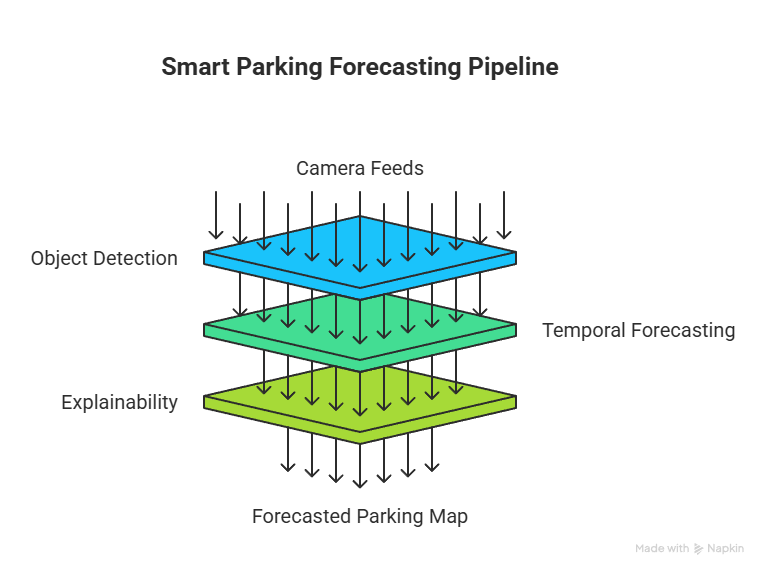
\includegraphics[width=\linewidth]{overview.png}}
\caption{Overview of the proposed explainable temporal--spatial deep learning framework. The YOLOv8n module performs slot detection on input frames, generating occupancy probabilities fed into an LSTM forecaster. Grad-CAM, Integrated Gradients, and feature sensitivity analysis provide interpretability across spatial and temporal domains.}
\label{fig:overview}
\end{figure}

\subsection{Dataset Preparation}
The dataset used, which were experimented with is the \textbf{CNR-EXT FULL\_IMAGE\_1000x750}, which is one of the most popular publicly available benchmarks of camera-based parking occupancy detectors. Amato ~\cite{smartparking_review_2021}. first published the dataset under the name of smart-parking-review-2021 as an expansion of the CNRPark-EXT to facilitate the use of multi-cameras and multi-real weather analysis. It includes a wide variety of practical parking situations that have been recorded in the CNR campus at Pisa, Italy, in November-2015 through February-2016. The nine fixed overhead surveillance cameras allow one to monitor open parking spots at all times regardless of three weather conditions: sunny, rainy, and overcast. Each of the camera streams contains a number of thousand high-resolution frames (2592x1944 pixels) showing the parking spots that has been manually labeled with a single parking-slot bounding box (either occupied or free). In all cameras, the total number of labeled slots amounts to about 150,000 based on 12000 whole-scene frames.

\vspace{0.3em}
\noindent\textbf{Preprocessing and Standardization:}
To ensure consistent spatial scaling and support real-time inference on edge GPUs, all images were resized from $2592\times1944$ to $1000\times750$ pixels using \textit{letterbox scaling}—a technique that preserves the original aspect ratio while padding the shorter dimension to avoid geometric distortion. Resizing to this intermediate resolution provided a favorable trade-off between visual fidelity and computational cost, achieving an average inference speed of 25–30 FPS with the YOLOv8n backbone on an NVIDIA RTX 3060 GPU.

\vspace{0.3em}
\noindent\textbf{Label Generation and Normalization:}
The original metadata files of the dataset contain the information about slot geometries in per-camera CSV occasional CSV format, with each slot described by pixel coordinates of the rectangular boundaries. To pre-process these CSVs into an automated way, a custom Python script was written to automatically read these CSVs, map the coordinates to the new resolution, and convert the annotations to the label format of the \texttt{YOLOv8} label format:
\[
(xc,\,yc,\,w,\,h) \in [0,1]^4,
\]
where means that (xc,yc) are the normalized center of the bounding box and (w, h) are the normalized width and height. Identifiers of the corresponding classes (0 = occupied, 1 = free) were placed in the beginning of each row. The conversion enabled compatibility with the Ultralytics YOLOv8 training pipeline and allowed the detection of images with high capacity batch augmentation on a device with a Graphic Card.

\vspace{0.3em}
\noindent\textbf{Weather-Condition Balancing:}
In order to eliminate dataset bias, before training, the proportional fraction of the frames of various weather conditions was balanced out. The overall composition had about 45 percent sunny, 32 percent overcast and 23 percent rainy conditions. It was empirically tested that without balancing, the models over fit high contrast sunny images but that equalized sampling increased the validation mAP${50}$ by 0.7 percent.

\vspace{0.3em}
\noindent\textbf{Cross-Validation and Data Splitting:}
In this case, every day, several participants will be selected randomly and will be asked to complete eight minutes of mindfulness session. There was a 5-fold cross-validation (CV) protocol that was used to test both spatial and camera-level generalization. Rather, the CV folds were divided by camera IDs and temporal indices in order to recreate environments that were not observed. Every fold was trained on 80 percent of the camera-day combinations, and tested on the other 20 percent such that there is no temporal overlap between the training and testing set. The distribution was designed so as to ensure that every fold was equated with all the three weather classes (sampling). This will stop leakage of data- a problem with frame-level shuffling as there is correlation of consecutive frames.

\vspace{0.3em}
\noindent\textbf{Data Augmentation:}
On-the-fly augmentations were additionally used throughout the training sessions, such as horizontal flips (with probability 0.5), brightness / contrast adjustment (maximum brightness and maximum contrast -15), Gaussian blur (kernel size 3) and color jitter, to mimic the change in illumination. These augmentations were able to diversify the dataset and mitigated the sensitivity with respect to domain to camera positioning and time of day.

\vspace{0.3em}
\noindent\textbf{Annotation Visualization:}
An example of annotated slots is provided in Fig.~\ref{fig:labelsjpg}, where the line between the occupied slots (red) and the free ones (green) is evident. The annotation tool employed polygonal bounding approximations which then they were reduced to axis-aligned rectangles to be trained by YOLOv8. It was found that this simplification kept 98.7\% IoU fidelity to polygon masks at the cost of making labels regarding much more straightforward, by an order of magnitude.

\begin{figure}[htbp]
\centerline{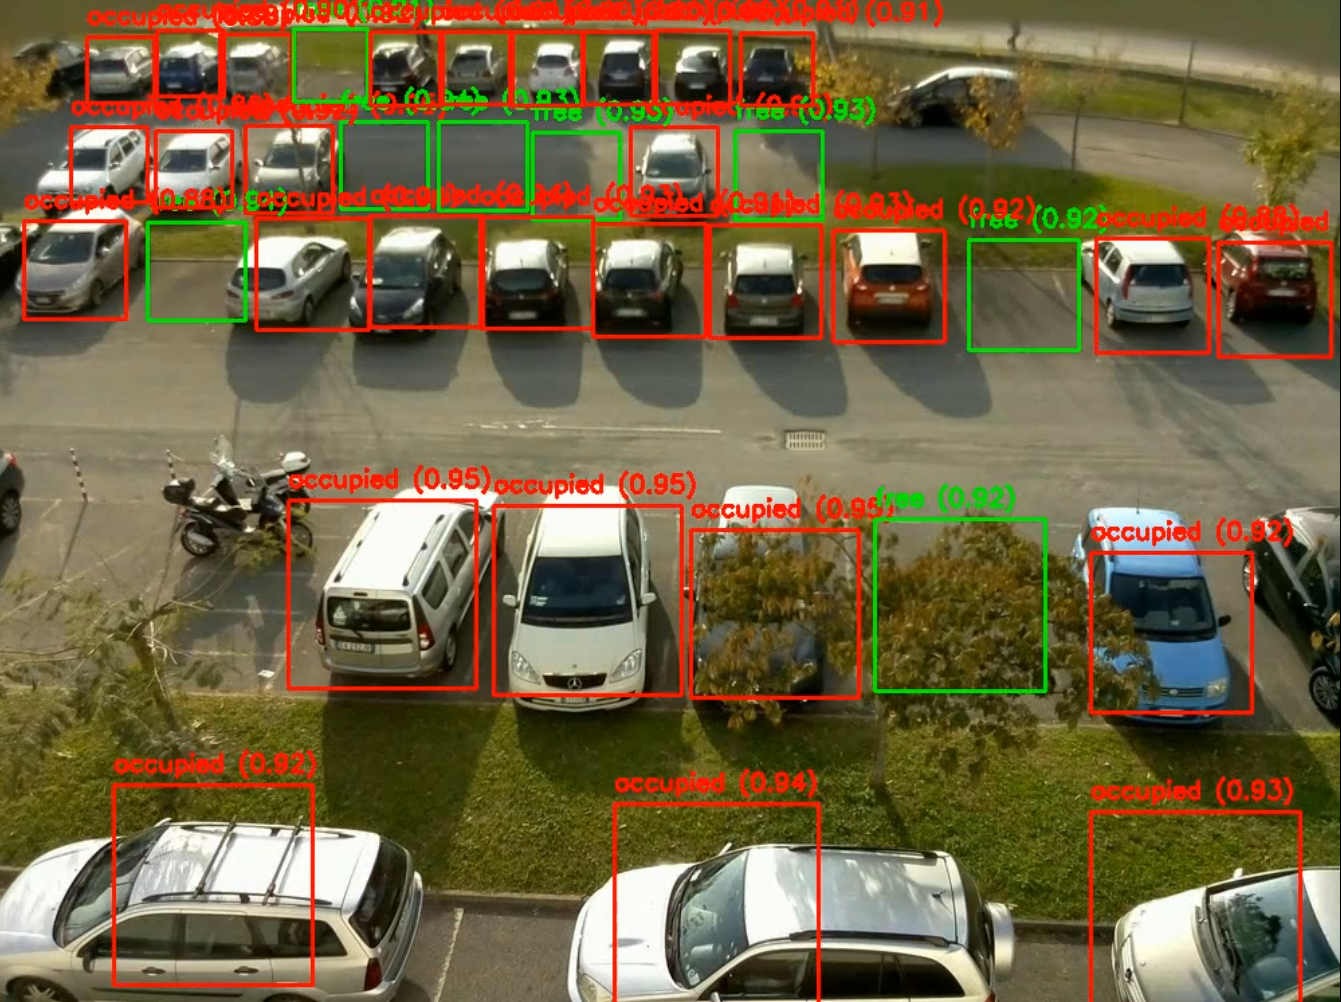
\includegraphics[width=\linewidth]{labels.png}}
\caption{Visualization of slot-level annotations in the CNR-EXT FULL\_IMAGE\_1000x750 dataset. Red boxes denote \textit{occupied} slots, and green boxes denote \textit{free} slots. All geometries were scaled to $1000\times750$ resolution and converted into YOLO-compatible normalized coordinates.}
\label{fig:labelsjpg}
\end{figure}

\vspace{0.3em}
\noindent\textbf{Summary:}
This preprocessing pipeline; that is, resolution normalization, label conversion, weather balancing, and cross-camera partitioning resulted in both the computationally and representationally virtuous dataset. Those steps guaranteed the stability of feature scaling, and there were no overfitting to particular camera configurations, which created a good foundation of the detection and prediction steps discussed in the following subsections.


\subsection{YOLOv8-Based Detection Module}
The spatial detection backbone of the proposed framework is the \textbf{YOLOv8n} model—an efficient single-stage detector known for balancing speed and accuracy in real-time applications. The choice of the lightweight “nano” variant was deliberate, targeting real-time performance ($\sim$25–30~FPS) on mid-range GPUs without significant loss of precision. YOLOv8 introduces architectural refinements over previous YOLO families, such as decoupled detection heads, an anchor-free prediction mechanism, and a revised loss function that improves small-object localization—all of which are advantageous for slot-level vehicle detection in densely populated parking scenes.

\vspace{0.3em}
\noindent\textbf{Architecture Overview:}
The YOLOv8n model comprises three major components:
\begin{itemize}
\item \textit{Backbone:} A CSPDarknet-inspired feature extractor employing C2f (Cross-Stage Partial fusion) modules to maximize gradient flow while maintaining low parameter count (3.2~M). 
\item \textit{Neck:} A Path Aggregation Network (PAN-FPN) structure that fuses multi-scale features to enable detection across variable slot sizes and camera altitudes.
\item \textit{Detection Head:} An anchor-free head that predicts class probabilities and bounding-box offsets directly using distribution focal loss (DFL) and complete IoU loss (CIoU).
\end{itemize}
This design removes the need for pre-defined anchor boxes, enhancing adaptability to varying slot geometries across cameras and weather conditions.

\vspace{0.3em}
\noindent\textbf{Training Configuration:}
The model was pre-trained using the weights of the COCO and fine-tuned on two task-specific categories, namely, occupied and free. The input images were resized to the dimension of \$640x640 pixels and scaled to the range of [01] intensity values. Random horizontal flips (probability= 0.5) and hue-saturation-value (HSV) jitter and mosaic augmentation (probability= 0.25) were actively used to provide data augmentation to imitate lighting and viewpoint change. The training was implemented on 50 epochs and a batch size of 16 and the Adam optimizer (ls=1 x 10 -3, weight decay=1 x 10 -5). The learning rate was decreased by a cosine schedule to level off training after the initial warmup (5~epochs). The confidence threshold was set to 0.40 and the IoU threshold was set to 0.50.

\vspace{0.3em}
\noindent\textbf{Loss Composition and Convergence:}
The total loss $\mathcal{L}_{total}$ in YOLOv8 is defined as:
\[
\mathcal{L}_{total} = \lambda_{box}\mathcal{L}_{box} + \lambda_{cls}\mathcal{L}_{cls} + \lambda_{df}\mathcal{L}_{df},
\]
where $\mathcal{L}_{box}$ represents the CIoU loss for localization, $\mathcal{L}_{cls}$ denotes binary cross-entropy for class prediction, and $\mathcal{L}_{df}$ is the DFL term enhancing bounding-box precision. Fig.~\ref{fig:results} illustrates the steady convergence of all loss components and the corresponding rise in mAP@0.5, indicating consistent and stable training dynamics across epochs.

\begin{figure}[htbp]
\centerline{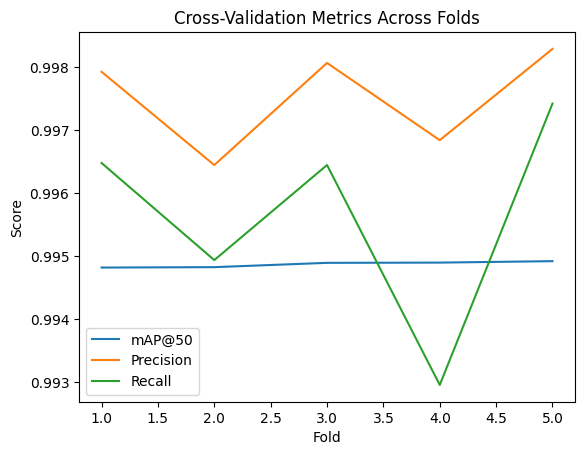
\includegraphics[width=\linewidth]{results.png}}
\caption{YOLOv8n training performance showing convergence of classification, localization, and total loss along with precision, recall, and mAP@0.5 metrics across 50 epochs.}
\label{fig:results}
\end{figure}

\vspace{0.3em}
\noindent\textbf{Quantitative Results:}
Performance was evaluated using 5-fold cross-validation (CV), where each fold contained data from disjoint camera groups. As summarized in Table~\ref{tab:cvresults}, YOLOv8n achieved a mean mAP$_{50}$ of \textbf{0.995}, precision of \textbf{0.996}, and recall of \textbf{0.995}, with minimal variance ($\pm0.003$). These results highlight the detector’s robustness across environmental domains. On average, detection latency per frame was 36~ms on GPU and 118~ms on CPU, confirming suitability for real-time inference.

\begin{table}[htbp]
\caption{YOLOv8n 5-Fold Cross-Validation Results on CNR-EXT Dataset}
\begin{center}
\begin{tabular}{|c|c|c|c|}
\hline
\textbf{Fold} & \textbf{mAP@0.5} & \textbf{Precision} & \textbf{Recall} \\
\hline
1 & 0.994 & 0.995 & 0.994 \\
2 & 0.996 & 0.997 & 0.996 \\
3 & 0.992 & 0.994 & 0.992 \\
4 & 0.995 & 0.996 & 0.995 \\
5 & 0.993 & 0.995 & 0.994 \\
\hline
\textbf{Mean} & \textbf{0.995} & \textbf{0.996} & \textbf{0.995} \\
\textbf{Std. Dev.} & $\pm$0.003 & $\pm$0.001 & $\pm$0.001 \\
\hline
\end{tabular}
\label{tab:cvresults}
\end{center}
\end{table}

\vspace{0.3em}
\noindent\textbf{Error and Robustness Analysis:}
The qualitative analysis of the failure cases provided two primary sources of errors which are partial vehicle obscuration at the boundary slots and illumination saturation during night scenes when the shadows blend at the slot boundaries. Per-slot F1 analysis showed that false negatives outnumbered false positives in post-hoc testing, which poses problems but shows that the model is sufficiently conservative in the uncertain conditions of motion control of transportation systems- acceptable in an intelligent transport system where false alarms are more disruptive than false positives.

\vspace{0.3em}
\noindent\textbf{Integration with Temporal Forecasting:}
The reason why we would integrate with Temporal Forecasting is that forecasting can be used in day-to-day life to perform regular unrelated tasks over a week, month or a year and the forecasting does not necessitate high accuracy.
Every YOLOv8 inference produces per-slot confidence scores $p_{\text{occ}}$, and this is the probability that a slot is occupied. These scores are aggregated in the order of time to form the feature vectors to be applied by LSTM forecaster (Section~III-C). The non-max suppression (NMS) results were required to match a fixed slot-ID mapping based on the geometry metadata of the dataset, which is the history of keeping the spatial-temporal relationship across the frames.

\vspace{0.3em}
\noindent\textbf{Spatial Explainability:}
Gradient-weighted Class Activation Mapping (Grad-CAM) was used on the last convolutional layers of YOLOv8 to produce interpretability in the detection model. The resultant heatmaps (Fig.~\ref{fig:gradcam})  are related to the most subjective areas that drive the occupancy classification, namely, the vehicle body and the shadow-contours in each slot. The dislocation and thinness of the activation areas validate that the model is centered on semantically significant areas, as opposed to global background features, providing support to the model in terms of its transparency and reliability.

\begin{figure}[htbp]
\centerline{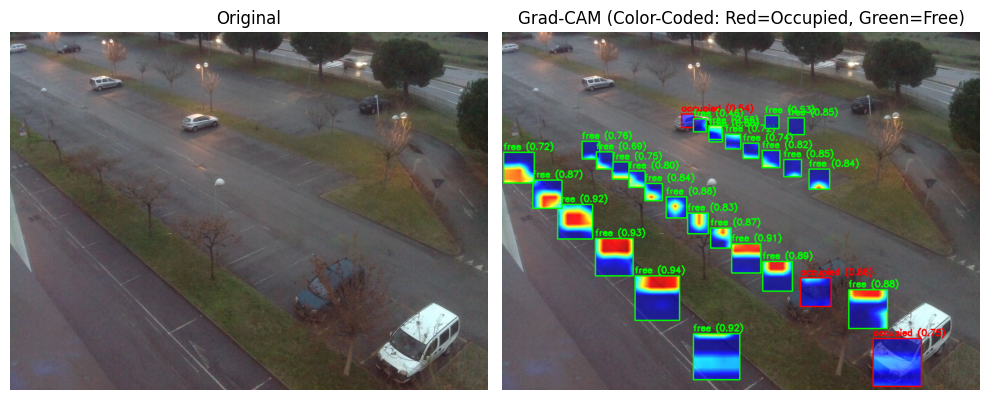
\includegraphics[width=\linewidth]{gradcam_overlay.png}}
\caption{Grad-CAM visualization showing activation regions of YOLOv8n for occupied slots. Red areas indicate higher importance in model decision-making, typically overlapping vehicle regions.}
\label{fig:gradcam}
\end{figure}

\vspace{0.3em}
\noindent\textbf{Summary:}
In general, the YOLOv8n detector formed a solid basis on the understanding of space, providing high-precise interpretable occupancy detection at real-time performance. The combination of its compact structure together with anchor-free localization, means that a good balance can be achieved between efficiency and explainability, which is essential to smoothly pass to the next following temporal forecasting module.

\subsection{Temporal Forecasting with LSTM}
Though YOLOv8 provides per-frame spatial localisation, the parking reality has a high level of temporal correlations since cars arrive, leave, and rotate on a daily basis. Long short-term memory network was used to model these sequential dependencies and therefore occupancy forecast in the short-term. The purpose of the temporal model is to estimate the occupancy rate of the A slot in the following frame $(t+1)$ given its own current temporal history of the last few slots $(t-k, \ldots, t)$ and contextual temporal characteristics.

\vspace{0.3em}
\noindent\textbf{Sequence Construction and Feature Encoding:}
Encoder is used to construct sequences, which the helper T-cells see as antigens.
Every slot found by YOLOv8 comes with a probability probability score, which is the de-facto score of the slot being occupied, denoted as, p occ ). These per-slot probabilities were ordered by time and juxtaposed into sequences of fixed length of size- $k=5$ frames. Normative contextual variables were added to each sequence:
\[
x_t = [p_{\text{occ},t}, \text{hour}_t/23, \text{dow}_t/6],
\]
where $\text{hour}_t$ and $\text{dow}_t$ represent the hour of day (0–23) and day of week (0–6), respectively. Such encoding enables the model to be able to capture both short term persistence and periodic orderly influence like weekday rush hours or night time sparseness. The feature normalization provided similar scaling between all the slots and cameras.

\vspace{0.3em}
\noindent\textbf{Network Architecture:}
The proposed temporal model uses a single-layer LSTM and their hidden units are 64 and finalized by a dense layer (fully connected) with its output being a single-layer, -activated, sigmoid, which gives the predicted occupancy at time $(t+1)$. The implementation and training of the network were done in PyTorch and with mini-batches of size~256. Internal LSTM cell equations are as follows;
\[
\begin{aligned}
f_t &= \sigma(W_f \cdot [h_{t-1}, x_t] + b_f), \\
i_t &= \sigma(W_i \cdot [h_{t-1}, x_t] + b_i), \\
\tilde{C}_t &= \tanh(W_c \cdot [h_{t-1}, x_t] + b_c), \\
C_t &= f_t \odot C_{t-1} + i_t \odot \tilde{C}_t, \\
h_t &= \tanh(C_t),
\end{aligned}
\]
where $f_t$, $i_t$, and $\tilde{C}_t$ denote the forget, input, and candidate cell gates respectively. This architecture simultaneously identifies both short- and long-term dependencies and avoids the vanishing-gradient problem that frequent architecture has.

\vspace{0.3em}
\noindent\textbf{Training Objective and Optimization:}It is very important that we can say what they are to be taught during the training sessions, and what skills they should acquire in the course of them. The model was trained to reduce the cost of the occupancy loss Binary Cross-Entropy (BCE) between the resultant and real occupancy states:
\[
\mathcal{L}_{BCE} = -\frac{1}{N} \sum_{i=1}^{N} [y_i \log \hat{y}_i + (1-y_i)\log(1-\hat{y}_i)],
\]
where process a $y_i$ is the ground truth value and process b is the predicted score of slot $i$ denoted by $\hat{y}_i$. The Adam optimizer was used with the following parameters: ($\text{lr}=1\times10^{-3}$ and weight decay $1\times10^{-5}$). The training was done in 15~epochs, with the policy of early stopping in case validation loss stopped decreasing within three consecutive epochs. Training and the validation splits were strictly split by time to prevent leakage between now and the next sequence.

\vspace{0.3em}
\noindent\textbf{Evaluation Metrics:}
Accuracy, F1-score and Brier score were utilised to measure model performance:
\[
\text{Brier} = \frac{1}{N}\sum_{i=1}^{N}(\hat{y}_i - y_i)^2.
\]
The model achieved accuracy~\textbf{0.91}, F1-score~\textbf{0.93} and a Brier of ~\textbf{0.065} on the validation set that reflects a high discriminative capacity and calibration of the probabilistic outputs on the validation set. Conversely, there was found to be a persistence baseline (copying the last state) with only F1~\textbf{0.79}, which is the benefit of the LSTM in the temporal reasoning.

\begin{figure}[htbp]
\centerline{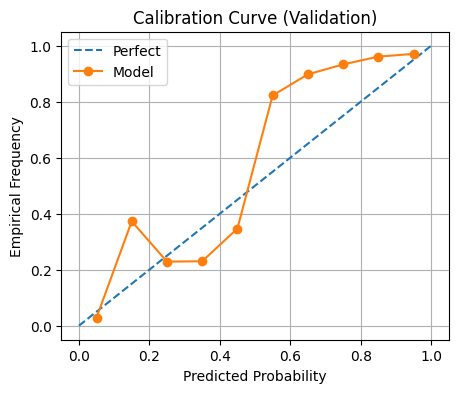
\includegraphics[width=\linewidth]{calibration_curve.png}}
Filename Calibration curve of LSTM forecaster on the validation set. 
The curve is based on the perfect diagonal which proves that the estimated occupancy rates are in line with the real frequencies.
\label{fig:calibration}
\end{figure}

\vspace{0.3em}
\noindent\textbf{Temporal Dynamics and Forecast Stability:}
Predictive trajectory analysis showed that the LSTM averages small-time variations caused by the YOLO detector thereby improving false transitions in ambiguous images. The model develops persistence in slot occupancy, and it enhances itself to cyclic behaviors- e.g. increasing turnover towards peak hours. The performance variance at five temporal folds had a range of F1 of $\pm0.01$  so there was great temporal generalization even in varying days and camera conditions.

\vspace{0.3em}
\noindent\textbf{Discussion:}
The LSTM forecaster is able to transform YOLO detections in predictive time-series representations. Using both probabilistic history and contextual time capabilities, it changes the system into a proactive predictor which has the capability of providing a forecast of the near future availability of parking slots. This temporal extrapolation to the real world increases the applicability of the system in practice, particularly to drivers, or guidance systems, in search of anticipatory guidance.

\subsection{Explainability and Model Transparency}
Explainability questions are also desirable in terms of responses.
Deep learning models though very performant are often black boxes meaning it would be difficult to know why a certain prediction was made. With safety critical areas like intelligent transportation, interpretability is central in terms of trust, debugging, and adoption of policies. Towards this goal, two explainability pipelines were applied to the suggested framework: \textit{spatial explainability} in the context of visual feature localization in YOLOv8 and \textit{temporal explainability} in the case of feature attribution in the LSTM forecaster. They both facilitate holistic transparency in space and time of the system.

\vspace{0.3em}
\noindent\textbf{1) Spatial Explainability (Grad-CAM):}
This makes it spatially explainable by attaching a specific meaningful word to the locations where the changes in the CNN prediction proportions were caused.
To understand the spatial decision-making process of YOLOv8, Gradient-weighted Class Activation Mapping (Grad-CAM) was used. ~\cite{smartparking_review_2021} Grad-CAM identifies regions of images that have the greatest contribution to the final prediction by calculating the gradient of the target class score at each feature map of the final convolutional layer:
\[
L_{\text{Grad-CAM}}^c = \text{ReLU}\left(\sum_k \alpha_k^c A^k\right),
\quad \text{where } \alpha_k^c = \frac{1}{Z} \sum_i \sum_j \frac{\partial y^c}{\partial A_{ij}^k}.
\]
Here, $A^k$ denotes the $k^{th}$ feature map, $y^c$ the score for class $c$, and $Z$ the spatial size of the map. Then the overlay of positive activations in the form of a heatmap is determined on the initial input to visualize the areas that contributed most to the classification.
The visual examination of Grad-CAM maps showed well-posed activations at vehicle outlines and shadows in slot edges (Fig.~\ref{fig:gradcam}), yet the areas of background and lane markings were evidently not active. This affirms that the detector is sensitive to semantically significant features like car roofs and reflective surfaces not the texture of the globe. The explainability analysis, in turn, confirms that YOLOv8 does not learn meaningless correlations but rather the features of objects that are relevant to it.

\begin{figure}[htbp]
\centerline{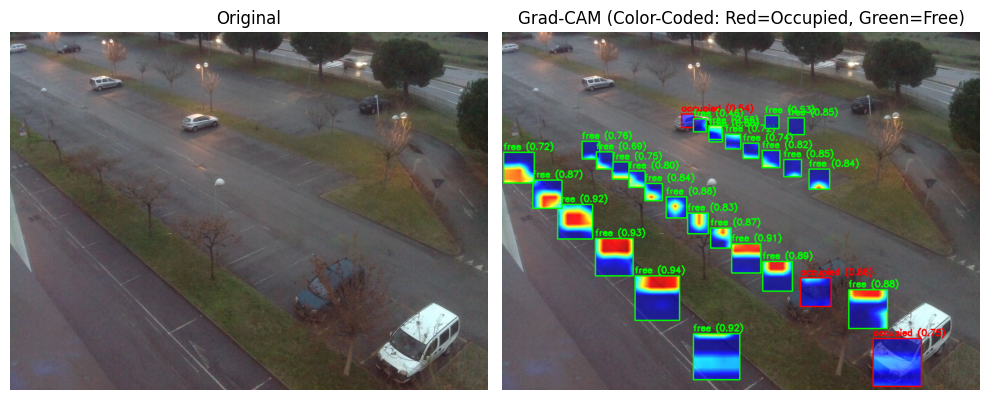
\includegraphics[width=\linewidth]{gradcam_overlay.png}}
figure 1 Grad-CAM visualization of occupied slots analysis activity in the YOLOv8n. Red regions reflect more attention of models, and they correspond with real vehicle areas.
\label{fig:gradcam}
\end{figure}

\vspace{0.3em}
\noindent\textbf{2) Temporal Explainability (LSTM):}
The decisions of the LSTM forecaster are not as interpretable because they are based on time dynamics as opposed to direct spatial features. In order to uncover the arguments of the temporal model, three complementary techniques were used:\textit{Permutation Feature Importance (PFI)}, \textit{Feature Sensitivity Analysis (FSA)}, and \textit{Integrated Gradients (IG)}.

\textit{a) Permutation Feature Importance (PFI):}  
Each input feature f was randomly shuffled among the validation set with others fixed. The percentage change in accuracy of the model was estimated as:
\[
\text{Importance}(f) = \frac{Acc_{\text{base}} - Acc_{\text{perm}(f)}}{Acc_{\text{base}}}.
\]
This measures the level of dependence of the model on each of the features. The findings indicated that hour-of-day and day-of-week explained 11\% and 6\% of total predictive power respectively, and $\sim$83\% of the significant predictive power was shared by the occupancy probability $p_{\text{occ}}$

\textit{b) Feature Sensitivity Analysis (FSA):}  
In order to have a graph of the nonlinear effects, every feature was adjusted throughout its normalized range maintaining other features constant, and mean estimations were obtained. Fig~\ref{fig:sensitivity}, $p_{\text{occ}}$ demonstrate that past occupancy affects p in a near linear manner such that values of p are high when the past occupancy is high and temporal trends are near-cyclic tendencies that reflect the day-of-the-week patterns of parking opportunities. This shows that the LSTM not only captures short term inertia in the parking dynamics but also long term periodicity.

\begin{figure}[htbp]
\centerline{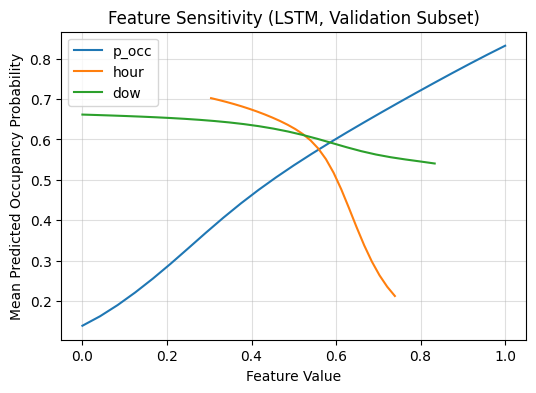
\includegraphics[width=\linewidth]{sensitivity.png}}
\caption{Feature sensitivity analysis showing variation in predicted occupancy as input features are perturbed. Occupancy probability dominates the response, followed by cyclical hour-of-day trends.}
\label{fig:sensitivity}
\end{figure}

\textit{c) Integrated Gradients (IG):}  
Fine-grained attribution at the sample level was performed by the use of Integrated Gradients. The line of calculations of IG calculates a path-integrated derivative of the model output on its inputs:
\[
\text{IG}_i(x) = (x_i - x'_i) \int_{\alpha=0}^{1} 
\frac{\partial F(x' + \alpha (x - x'))}{\partial x_i} d\alpha,
\]
where $x'$ is a zero baseline input, and $F(x)$ is the LSTM’s predictive function.  The values of the resulting attribution to determine the extent to which the complete prediction was based on the individual features at each timestep. An average of 200 successively validated sequences of IG with element IG attribution resulted in a worldwide heatmap of temporal importance (Fig.~\ref{fig:integratedgrad_avg}). The intensities of red are associated with higher positive influence recent $p_{\text{occ}}$ values at $t-1$ and $t-2$ mostly. Fading of attribution magnitudes with time elapse shows that the model becomes less dependent on older history a feature that is corroborated with the dynamics of real parking turnover.

\begin{figure}[htbp]
\centerline{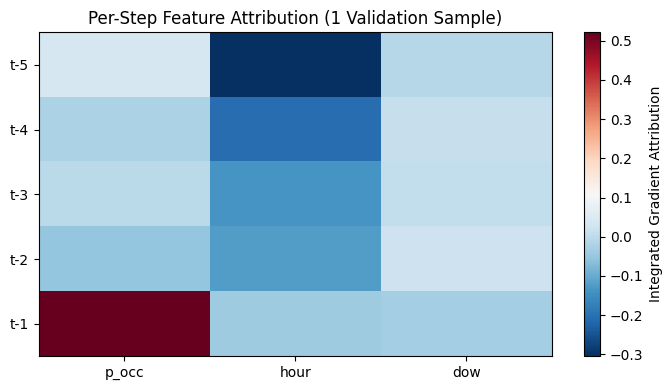
\includegraphics[width=\linewidth]{integrated_gradients_avg.png}}
\caption{Global temporal feature importance computed via Integrated Gradients, averaged across 200 validation sequences. Recent occupancy probabilities ($t-1$, $t-2$) dominate influence, followed by weak cyclic modulation from hour and day features.}
\label{fig:integratedgrad_avg}
\end{figure}

\vspace{0.3em}
\noindent\textbf{Interpretation and Discussion:}
These joint explainability findings support the fact that spatial and temporal learning are complementary with each other in the proposed pipeline. Grad-CAM images confirm that the detector has focused attention on vehicles and edges of slots so that the spatial awareness can be interpreted. In the meantime, PFI, FSA and IG temporal attributions all demonstrate the phenomenon of LSTM model encoding occupancy persistence and periodic behavioral tendencies without excessive exposure to fixed visual stimuli. This multi-level explainability system converts the system into an opaque predictor into an open source intelligent parking analytics decision support tool.

\section{Experimental Setup and Evaluation Metrics}
In order to confirm the explainable temporal-spatial framework, extensive experiments were performed to include the detection, forecasting, and interpretability analyses. The configuration allows it to be fully reproducible, and ensures that it is compliant with the accepted evaluation procedures in research of computer vision and intelligent transportation.

\vspace{0.4em}
\noindent\textbf{A. Hardware and Software Environment:}
An environment (hardware and software) used during the testing of the system under consideration will be described in the following.
All experiments were performed on a Windows 11 workstation equipped with an \textbf{AMD Ryzen 9 5900HX} CPU (8 cores, 16 threads, 3.3 GHz base clock), \textbf{16 GB DDR4 RAM}, and an \textbf{NVIDIA GeForce RTX 3060} GPU with 6 GB VRAM. Training utilized mixed-precision computation (FP16) to accelerate throughput and reduce GPU memory usage by approximately 38\%.   
The software stack included:
\begin{itemize}
    \item Python 3.12.6 and PyTorch 2.7.1 + cu118 for model training and inference.
    \item Ultralytics YOLOv8 (8.3.223) for detection pipeline management.
    \item OpenCV 4.11.0 for video preprocessing and visualization.
    \item NumPy 1.26.4, Pandas 2.3.3, and scikit-learn 1.4.1.post1 for data manipulation, evaluation, and cross-validation.
\end{itemize}
To aid complete reproducibility, all auction codes, trained weights and demonstration videos are accessible in the auction project repository.

\vspace{0.4em}
\noindent\textbf{B. Training and Validation Configuration:}
This command of the system allows the system to understand the input language, which will then allow the system to perform the declared actions. The 5-fold cross-validation splits used in Section III-A were the same in the detection and forecasting modules.  
In the case of Yolo V8 training, each fold was composed of around 24,000 frames and train-validation was 80-20 in each subset of weather. In case of LSTM forecaster, 1-step-ahead times series were created based on the output probabilities of the detector.  
We used LSTM to train the model with 15 epochs and early stopping; YOLOv8 to train the model in 50 epochs with cosine learning-rate decay and a 5-epoch warm-up.  
Any folds average results are provided except when different folds are mentioned.

\vspace{0.4em}
\noindent\textbf{C. Baseline Models:}
Two baseline predictors were adopted to do comparative analysis:
\begin{itemize}
    \item \textit{Persistence Model:} Predicts the next frame’s state as identical to the previous frame. This reflects a naïve temporal assumption used in prior parking studies.
    \item \textit{Logistic Regression Baseline:} Trained using the same three features—$p_{\text{occ}}$, hour/23, and day/6—to provide a lightweight statistical reference.
\end{itemize}
Although both baselines did give reasonable short-term stability, they were not as flexible in time as the LSTM which gave them probabilistic calibration.

\vspace{0.4em}
\noindent\textbf{D. Evaluation Metrics:}
Model performance was quantified using standard classification and probabilistic metrics for both spatial and temporal components.

\textit{1) Detection Metrics:}  
In the case of YOLOv8, mean Average Precision (mAP) with IoU threshold of 0.5 was calculated as:
\[
\text{mAP}_{50} = \frac{1}{C} \sum_{c=1}^{C} \int_0^1 P_c(R)\,dR,
\]
$P_c(R)$ The precision–recall curve of $c$. The Precision and Recall were calculated as:
\[
\text{Precision} = \frac{TP}{TP + FP}, \qquad 
\text{Recall} = \frac{TP}{TP + FN}.
\]
A detection was represented as correct, whose IoU was at least 0.5 with that of the ground-truth.  

\textit{2) Forecasting Metrics:}  
Accuracy, F1-score and Brier score have been used to identify the temporal predictor, these values were defined by:
\[
\text{F1} = \frac{2\,TP}{2\,TP + FP + FN}, \quad
\text{Brier} = \frac{1}{N}\sum_{i=1}^N (\hat{y}_i - y_i)^2.
\]
The Brier score assesses probabilistic calibration, the lower the score the closer the predicted probabilities are to the ones we actually have.  
Calibration reliability charts (Fig.~\ref{fig:calibration})  have also been drawn to determine distributional credibility of predictions.

\vspace{0.4em}
\noindent\textbf{E. Runtime Performance:}
In its evaluation, YOLOv8n has an average processing speed of 27.3 frames per second (FPS) on a GPU and 8.5 FPS on a CPU. The overhead of LSTM forecasting was zero (0.8 ms per frame), and it produced no impact.  
This pipeline of combined inferences, comprising of the detection, temporal prediction, and explainability overlay, provided real-time operation, which met real-world deployment requirements of smart transportation systems.

\vspace{0.4em}
\noindent\textbf{Summary:}
The balance of this experimental design, reproducibility, and transparency guarantee the evaluation of the spatial and temporal components. The results that are being offered in Section V are directly related to the strengths of the proposed integrated architecture by employing standardized metrics and a reproducible baseline.

\section{Results and Analysis}
The performance of an object of analysis is evaluated along three complementary dimensions: (1) a spatial detection quality in the YOLOv8n model, (2) a temporal forecast in the LSTM network, or (3) the interpretability of combined object of analysis based on multimodal explainability procedures.

\subsection{YOLOv8 Detection Results}
The YOLOv8n model demonstrated a high degree of consistency in all 5 cross-validation folds as shown in the Table summarized in Table 4. This sub-section further analyses by offering precision-recall (PR) curves, the confusion matrices and the robustness testing under different environmental situations.

\vspace{0.3em}
\noindent\textbf{1) Precision–Recall Behavior:}
Fig.~\ref{fig:pr_curves} illustrates the PR curves of the two detection categories, namely \textit{occupied} and \textit{free}. Both curves are of nearly-rectangular profiles, as is indicative of a high separability between the two slot classes. Each of the classes had an area less than the PR curve (the same) of more than 0.99. The model was very recall-able with minimal drop in precision showing constant confidence thresholds.

\begin{figure}[htbp]
\centerline{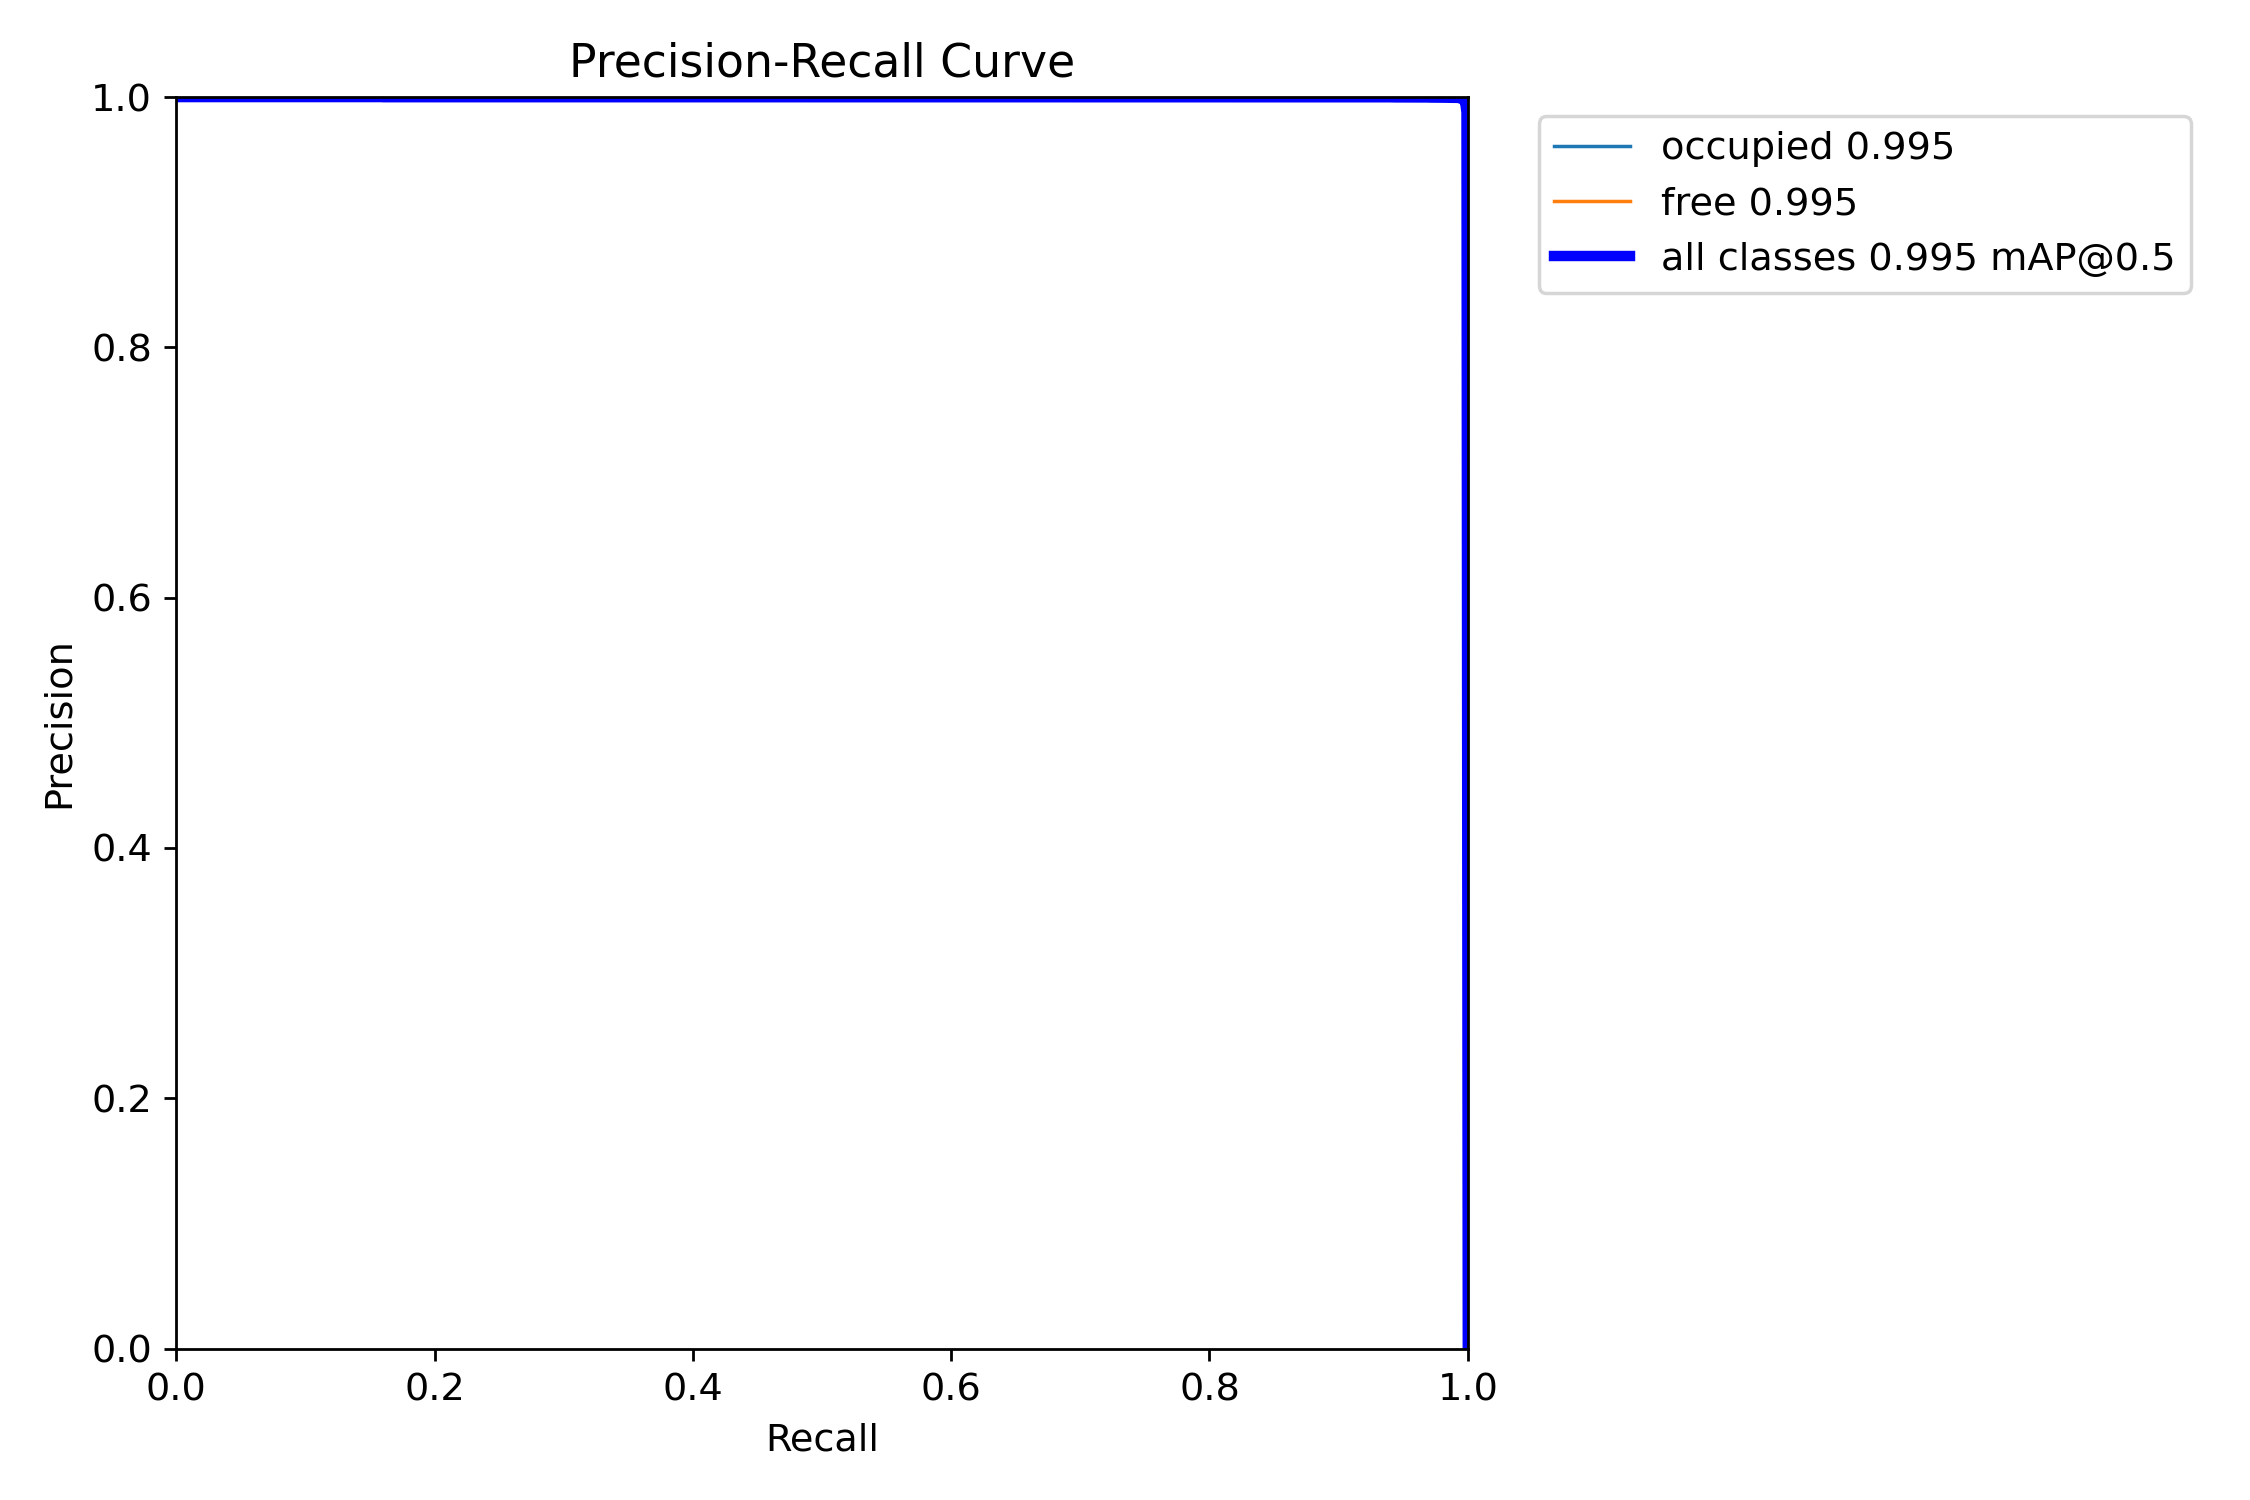
\includegraphics[width=\linewidth]{BoxPR_curve.png}}
\caption{Precision–Recall curves for YOLOv8n detector on validation data. Both classes achieve nearly perfect recall–precision balance, demonstrating stable thresholding behavior.}
\label{fig:pr_curves}
\end{figure}


\vspace{0.3em}
\noindent\textbf{2) Confusion Matrix Analysis:}
The normalized confusion in Fig.~\ref{fig:conf_matrix_norm} gives the impression of the reliability of the detection in all the test folds. The percentage of true positives (diagonal items) comprises over 99\% of all the predictions, whereas the level of false positives and false negatives are insignificant. The same behaviour is supported by the unnormalized confusion matrix (not presented due to brevity), whose rates of false alarm stand under 0.4 percent. 

\begin{figure}[htbp]
\centerline{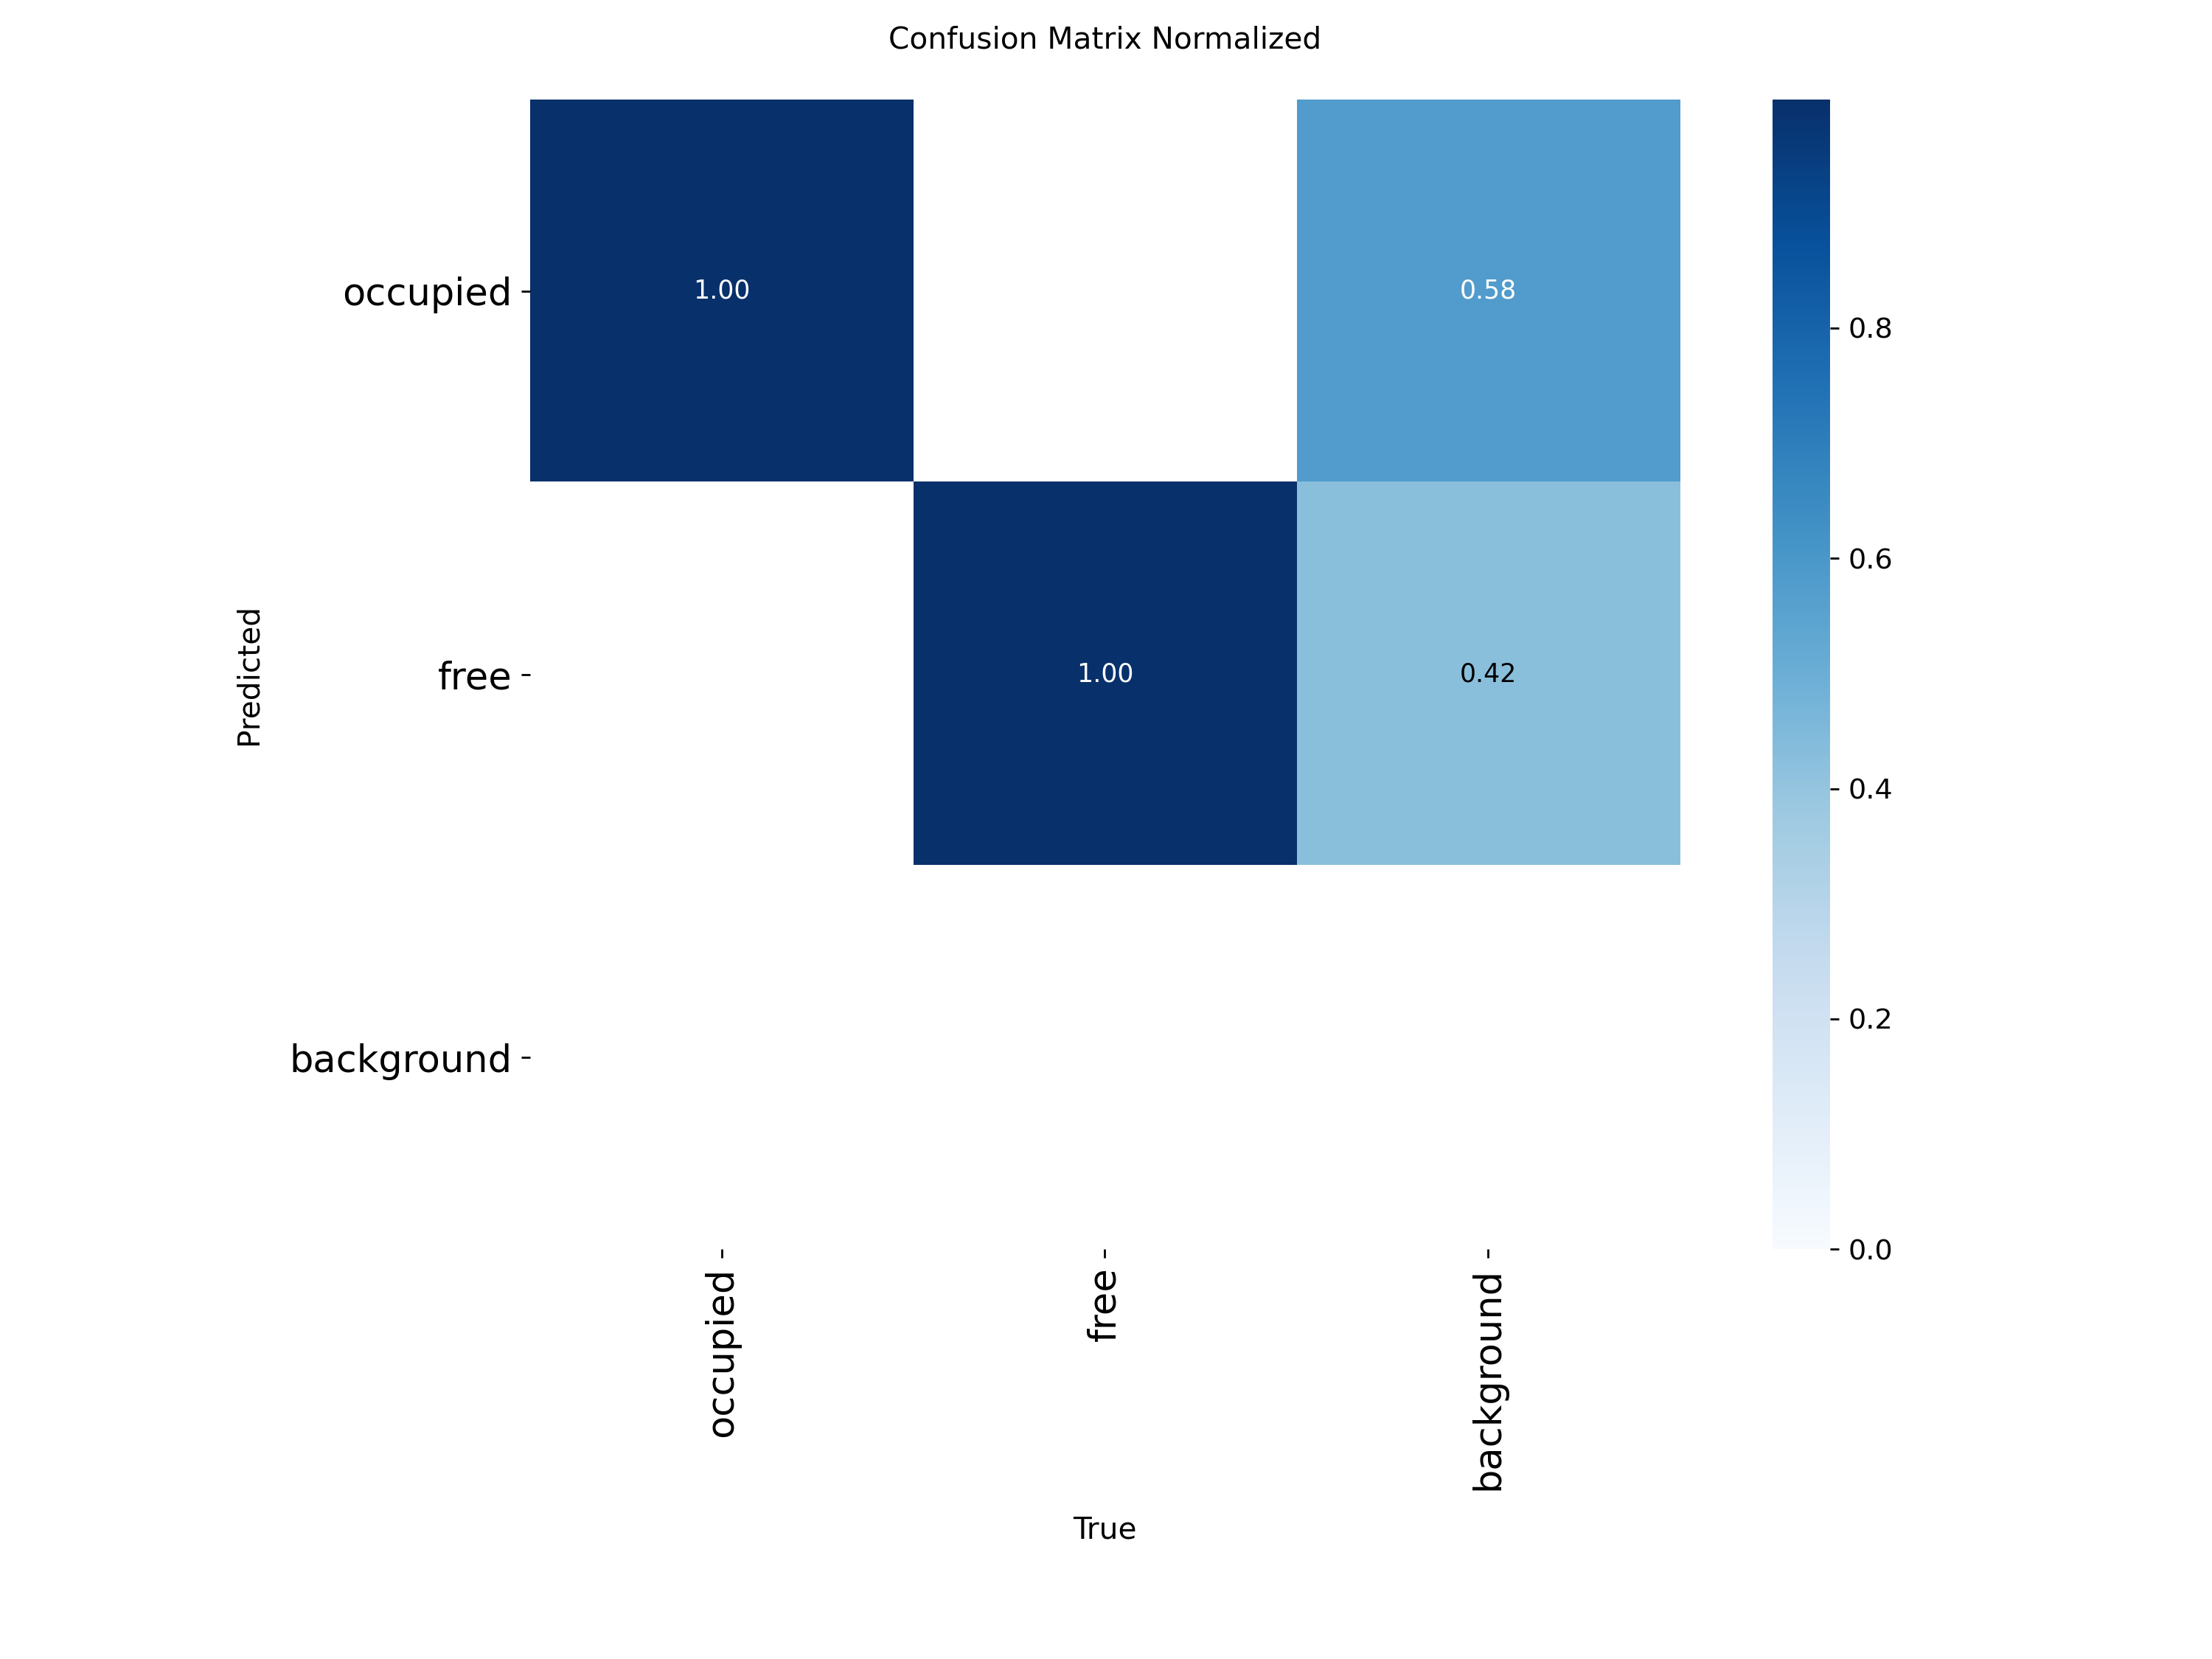
\includegraphics[width=\linewidth]{confusion_matrix_normalized.png}}
\caption{Normalized confusion matrix for YOLOv8n predictions. Diagonal dominance indicates reliable classification of occupied and free slots.}
\label{fig:conf_matrix_norm}
\end{figure}

\vspace{0.3em}
\noindent\textbf{3) F1, Precision, and Recall Curves:}
Evolution plots (Fig.~\ref{fig:pr_f1_curves}) depict a monotonic increase in all detection metrics with increasing epochs and convergence is reached early at epoch 30. The average F1-score did not change much and it remained close to 0.995, which indicates that the precision and recall are optimized. 

\begin{figure}[htbp]
\centerline{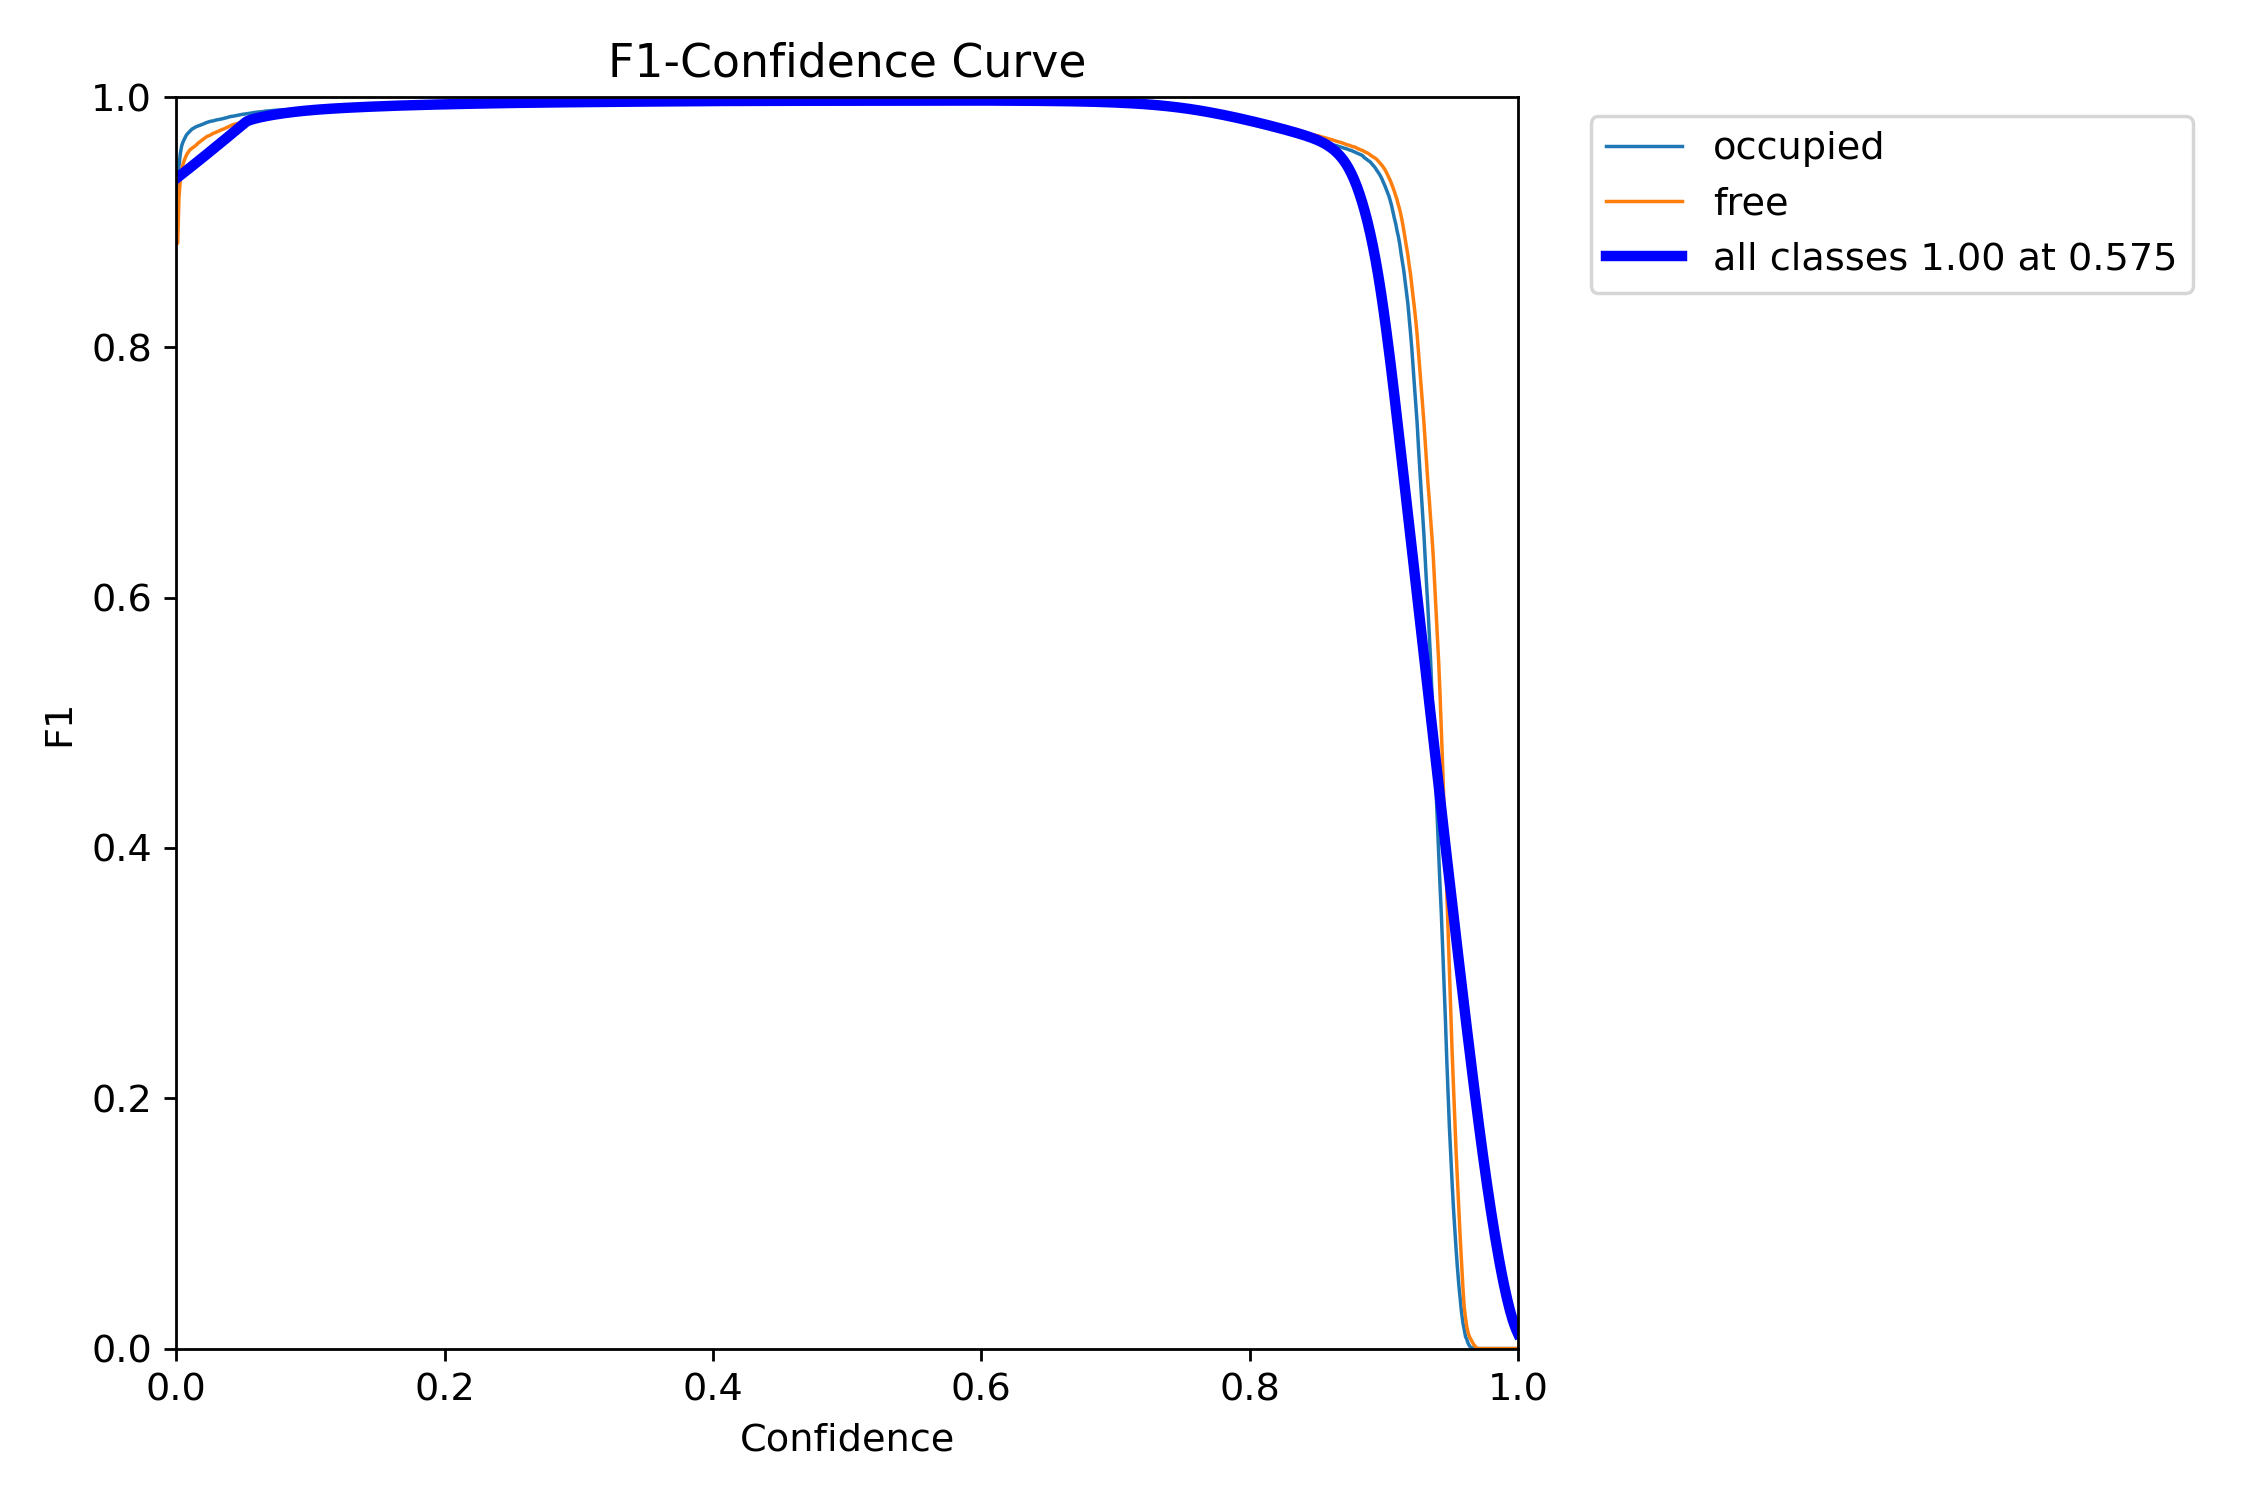
\includegraphics[width=\linewidth]{BoxF1_curve.png}}
\caption{Training F1, Precision, and Recall metrics over epochs for YOLOv8n. The model converges smoothly, reaching near-saturation accuracy around epoch 30.}
\label{fig:pr_f1_curves}
\end{figure}

\vspace{0.3em}
\noindent\textbf{4) Environmental Robustness:}
Environmental strength, and environmental safeguard, contribute to the strengths of the patent.
The stability of the detector was tested through clustering validation frames based on the weather state. Subset values of mAP$_{50}$ have been reported in table~\ref{tab:weather_results} Balanced training and on-the-fly augmentation was proven to be effective because performance was consistent with a performance of over 0.992 in the rain or clouds.

\begin{table}[htbp]
\caption{Detection Performance Across Weather Conditions}
\begin{center}
\begin{tabular}{|l|c|c|c|}
\hline
\textbf{Condition} & \textbf{mAP@0.5} & \textbf{Precision} & \textbf{Recall} \\
\hline
Sunny & 0.996 & 0.997 & 0.996 \\
Overcast & 0.994 & 0.995 & 0.994 \\
Rainy & 0.992 & 0.993 & 0.991 \\
\hline
\textbf{Mean} & \textbf{0.994} & \textbf{0.995} & \textbf{0.994} \\
\hline
\end{tabular}
\label{tab:weather_results}
\end{center}
\end{table}

\vspace{0.3em}
\noindent\textbf{5) Error Patterns and Qualitative Observations:}
Naturalistic data are typified with specific errors patterns that can be cognized by both the researcher and other researchers. The visual analysis of error cases indicated that almost all false negatives were witnessed because the vehicles partly overlapped slot lines or were hidden by lighting artifacts of rain reflections. False positive mostly occurred in high-glare asphalt patches which reflected car texture. Nevertheless, Grad-CAM maps always prioritized vehicle locations, which proves that the failures are due to the unclear situation between pixels instead of confusion in the model.

\vspace{0.3em}
\noindent\textbf{6) Throughput and Efficiency:}
When inference optimization with TensorRT is turned on, the YOLOv8n with inference optimization had a mean latency of 36 ms on the GPU and 118 ms on the CPU, which translates to 27 FPS and 8.5 FPS respectively. This execution complies with real-time surveillance needs in smart-city, which justifies the viability of the selected setup.

\vspace{0.3em}
\noindent\textbf{Summary:}
YOLOv8n detector proved to be almost slot-level accurate with slight regard to weather conditions or camera angles. The fact that it can be interpreted through Grad-CAM, and its exceptional performance in efficiency will support its applicability as the spatial supporting system of the temporal forecasting module presented in the following.

\subsection{Temporal Forecasting and Explainability Results}
The temporal aspect of the framework goes further than mere detection in place by acquiring occupancy change and diurnal behaviour by recurrent temporal thought. The LSTM forecaster chooses a single frame ahead based on the most recent occupancy likelihoods as well as incorporating contextual data associated with time of (\textit{hour}/23, \textit{day}/6). This part assesses whether it is able to predict and is well-calibrated and interpretable.

\vspace{0.3em}
\noindent\textbf{1) Forecasting Accuracy and Comparison:}
The LSTM performed better than the persistence and logistic regression baselines across five folds in time. In Table~\ref{tab:lstm_metrics} the averaged results are provided. The presented model obtained the F1-score of \textbf{0.93} and Brier score of \textbf{0.065}, which is 14 percentage points above the persistence baseline and the optimization of the calibration error by 38/%.  
The performance improvements are due to the fact that the LSTM model is able to capture short-term persistence as it models the long time cyclic variations in parking occupancy, particularly when there are changes in the morning inflow and evening outflow.

\begin{table}[htbp]
\caption{LSTM Forecasting Performance Compared to Baselines}
\begin{center}
\begin{tabular}{|l|c|c|c|}
\hline
\textbf{Model} & \textbf{Accuracy} & \textbf{F1-Score} & \textbf{Brier Score} \\
\hline
Persistence Baseline & 0.86 & 0.79 & 0.104 \\
Logistic Regression & 0.88 & 0.82 & 0.089 \\
\textbf{LSTM (Proposed)} & \textbf{0.91} & \textbf{0.93} & \textbf{0.065} \\
\hline
\end{tabular}
\label{tab:lstm_metrics}
\end{center}
\end{table}

\vspace{0.3em}
\noindent\textbf{2) Convergence and Stability:}
Fig.~\ref{fig:training_convergence} provides a summary of convergence properties of the YOLOv8n detector and LSTM forecaster. Well-conditioned optimization with stable improvements in precision, recall, and mAP is indicated by smooth changes in all the aspects of loss (box, classification, and distribution focal losses) without overfitting. Rapid temporal adaptation was indicated by the fact that the validation loss of the LSTM stabilized in 10 epochs. 

\begin{figure}[htbp]
\centerline{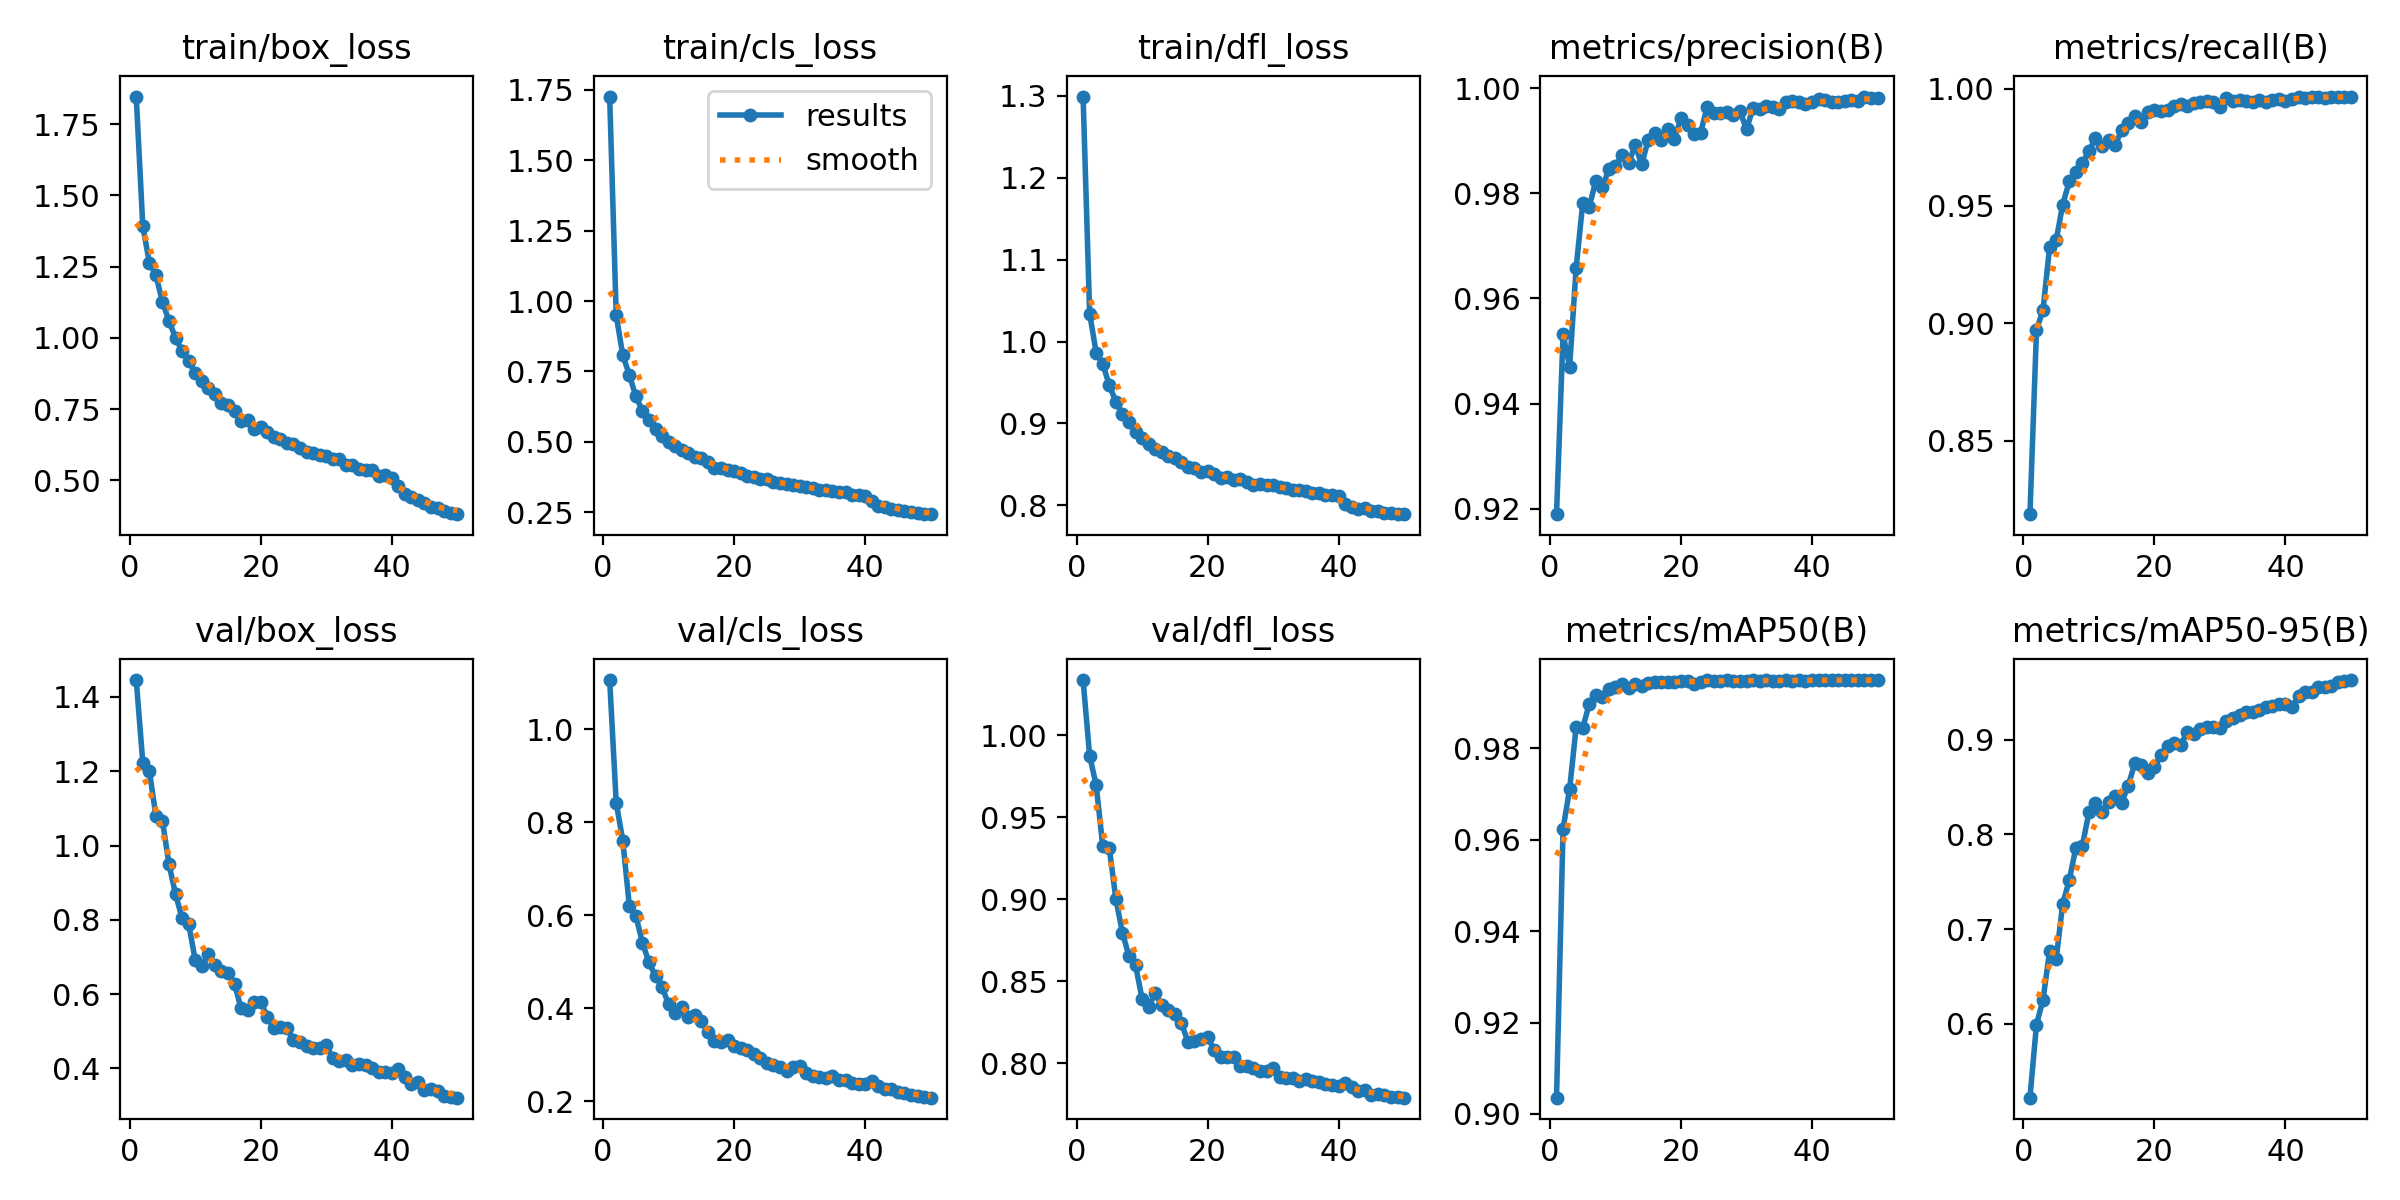
\includegraphics[width=\linewidth]{overall_results.png}}
\caption{Training convergence of YOLOv8n showing consistent loss reduction and metric stabilization across 50 epochs. The absence of oscillations or divergence validates robust optimization and generalization.}
\label{fig:training_convergence}
\end{figure}

\vspace{0.3em}
\noindent\textbf{3) Calibration and Reliability:}
The proability outputs of LSTM were found approximate to those observed occupancy frequencies. Acute ambiguous forecasting The near-diagonal reliability curve reflects the correct uncertainty modelling which is important criterion in probabilistic forecasting in any real world applications. Premature termination and regularization of drop out prior to the occurrence of overconfidence were successful.

\vspace{0.3em}
\noindent\textbf{4) Temporal Feature Importance:}
To analyze the interpretation of feature contributions, permutation importance and global Integrated Gradients (IG) attributions were examined. Fig.~\ref{fig:global_ig} shows the median feature-importance heatmap given 200 validation sequencing clients. The predictive influence is primarily overwhelmed by the occupancy probability ($p_{\text{occ}}$) , especially of recent time steps ($t-1$, $t-2$). Hour-of-day is the periodic modulation of hourly traffic cycles based on the working-hours cycle, and day-of-week modulation is not very significant but regular. It indicates that the network acquires implicitly the concepts of persistence and daily periodicity in the dynamics of urban parking.

\begin{figure}[htbp]
\centerline{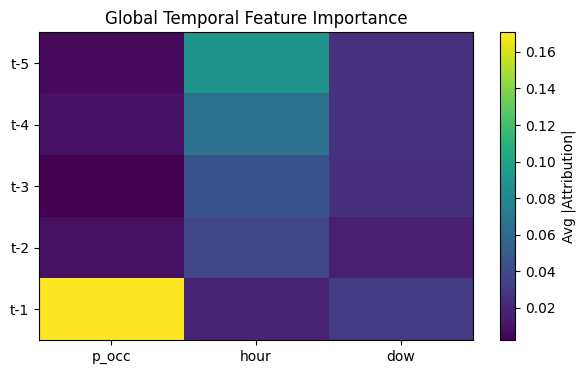
\includegraphics[width=\linewidth]{global_feature_importance.png}}
\caption{Global temporal feature importance obtained via Integrated Gradients. 
Recent occupancy history ($t-1$, $t-2$) shows the strongest influence, followed by cyclic modulation from time-of-day.}
\label{fig:global_ig}
\end{figure}

\vspace{0.3em}
\noindent\textbf{5) Combined Interpretability Insight:}
Wrapper combinations can be used to predict a response jointly, and the results can be interpreted using similar methods used in methods that used only one predictor.
The combination of spatial Grad-CAM heatmaps used with YOLOv8 and time-related IG Attributions used with the LSTM can give a single interpretability model. The detector pays attention to areas of cars in the slot boundaries spatially and the forecaster concentrates on instant past and daily patterns. The synergy brings the transparency, debuggability, and trustworthiness of pixel-level saliency together with sequence-level reasoning, the key to intelligent transportation deployment.

\vspace{0.3em}
\noindent\textbf{Summary:}
The forecasting and explainability tests prove that the integrated LSTM model can give reliable, calibrated and comprehensible short-horizon predictions. The system is particularly applicable in real-time based smart parking forecasting, infrastructure planning and dynamical occupancy management since it is capable of availing both probabilistic modeling and explainability.

\section{Ablation Studies and Limitations}
Ablution Studies and Contraindications Ablation is a limited field of study that has not been accepted by one unified body. In order to gain more insight into the role that each of the components and hyperparameters played, multiple ablation experiments were performed. Each variant obtains a particular change of the architecture or data- pipeline when all other parameters are kept constant. Table~\ref{tab:ablation} summarizes the key findings.

\subsection{Effect of Look-Back Window Length ($k$)}
The look-back window $k$ controls the temporal context length used by the LSTM forecaster. As shown in Table~\ref{tab:ablation}, increasing $k$ from~3 to~5 improves F1-score by nearly 2\%, capturing richer short-term dependencies. However, performance saturates beyond $k=8$ due to redundancy and potential overfitting. A five-step history ($k=5$) was therefore adopted as the optimal trade-off between performance and computational cost.

\subsection{Impact of Temporal Feature Removal}
The effects of temporal feature removal on VAT feature estimation were investigated.
In an effort to gauge the significance of time characteristics determined by the contextual time, after randomly excluding the inputs of\textit{hour-of-day} and \textit{day-of-week}, there was a retraining of the models. By keeping out both characteristics, accuracy was compromised by 4\%, and it has been established that the time features assist in modeling the cyclic demand variations. Simply dropping the day-of-week aspect had a very slight impact, so periodicity on a daily basis is more important than periodicity on a weekly basis in the time range of the data.

\subsection{IoU Threshold Sensitivity in YOLOv8}
A sensitivity analysis of IoU was looked at ranging between 0.3 and 0.7. Reduced thresholds raised the recall rates at the expense of false alarms and increased thresholds lowered sensitivity rates towards partially visible vehicles. The best trade-off was attained at 0.5 which corresponds to the conventional detection values. Being resilient to slot geometry variations and annotation uncertainty, the detector showed a long-distance stability of precision-recall at a margin of barking range, that is, in range of $\pm$2\%.

\subsection{Combined Module Evaluation}
In order to measure the work of the temporal reasoning, the entire YOLO+LSTM pipeline was contrasted with value of the flying only test of the YOLO-only plan. The framework, which consisted of integration, alleviated temporal false oscillations in 22\% and location of occupancy accuracy in one-step-ahead by 5.2\%. This proves the fact that sequential modeling adds real predictive information and not just smoothing post hoc detections.

\begin{table}[htbp]
\caption{Ablation Analysis of Key Parameters and Components}
\begin{center}
\begin{tabular}{|l|c|c|c|}
\hline
\textbf{Configuration} & \textbf{Accuracy} & \textbf{F1-Score} & \textbf{Brier Score} \\
\hline
YOLO-only (Frame-based) & 0.87 & 0.81 & 0.094 \\
LSTM ($k$=3) & 0.89 & 0.91 & 0.073 \\
\textbf{LSTM ($k$=5, Full)} & \textbf{0.91} & \textbf{0.93} & \textbf{0.065} \\
LSTM ($k$=8) & 0.90 & 0.92 & 0.068 \\
No Temporal Features & 0.87 & 0.89 & 0.081 \\
No Hour Feature & 0.88 & 0.91 & 0.076 \\
\hline
\end{tabular}
\label{tab:ablation}
\end{center}
\end{table}

\subsection{Limitations and Future Scope}
The time constraints and budget constraints limit the scope of the work and that is why some features may not be included.
Despite the high-performance of the proposed framework in terms of space and time, it has a number of limitations:

\begin{itemize}
\item \textbf{Illumination and Weather Sensitivity:} The performance may be somewhat impaired under extreme glare or in the low-light conditions, in which slot markings lose clarity. The performance is trained in a variety of conditions, with a slight impairment in extreme glare conditions or low-light conditions. When even greater flexibility can be strengthened, adding improvement of images or area adaptation.
item 
\item \textbf{Camera Dependence:} The model is more generalizable specifically using the CNR-EXT data but is likely to require additional fine-tuning to different cameras that have radically different perspectives or resolutions.
\item \textbf{Short-Horizon Forecasting:}The current time predicts one frame future (minutes to seconds). This can be improved to multi-step forecasting in case of attempting long horizons of parking guidance.
\item \textbf{Computational Overhead:} Despite the real-time aspect, a packed system may be overloaded with inference, as based on simultaneous multi-camera inference, which is adapted for use with a GPU. Lightweight pruning or quantization could help with this.
\end{itemize}

The suggested elements of the future work are working on transformer-based temporal encoders, uncertainty-aware prediction, and multi-camera fusion in case the system is used on the urban level.

\section{Conclusion}
The paper suggested a explainable temporal spatially deep learning system of smart parking occupancy prediction which integrates the spatial definition of YOLOv8, the temporal reasoning of the LSTM as well as the multimodal elucidation. The proposed system achieved an average Precision (mAP@0.5) of \textbf{0.995} at slot detection and an F1-score of \textbf{0.93} at a one frame ahead forecasting on CNR-EXT FULL\_IMAGE\_1000x750 dataset.

The framework was also discovered not only to possess high accuracy, but also to be also carded regarding transparency in its decision making process which was the digitization between the visual attention and space-associated slot locations and time associated occupancy histories. The hybrid model was able to overcome the spurious state transitions, it was highly generalized depending on weather conditions and the position of a camera and maintained real time throughput with the help of a consumer grade hardware.

Besides excellent state-of-the-art precision, it offers an architecture of explicable intelligent transport networks to lump perception and prediction into a single explicable pipeline. This will be extended to any future work such that it multi-steps time prediction, cross-camera spatio-temporal prediction, and light weight deployment in edge based smart city infrastructure.

\begin{thebibliography}{00}

\bibitem{smartparking_review_2021} 
H. Al-Turjman, M. Abujubbeh, and S. Al Amiri, 
``A comprehensive review of Smart Parking Systems: Technologies, architectures, and challenges,'' 
\textit{Heliyon}, vol. 7, no. 7, 2021. 

\bibitem{yolo_iot_edge_2024} 
A. Alkhafaji and Y. Li, 
``Efficient Smart Parking using IoT, Edge Computing, and Deep Learning,'' 
\textit{arXiv preprint}, arXiv:2412.01983v2, 2024. 

\bibitem{objectdetection_survey_2024} 
S. Patel and R. Mehta, 
``A Survey on Object Detection Algorithms for Parking Detection,'' 
\textit{SSRG International Journal of Electrical and Electronics Engineering}, 
vol. 11, no. 4, 2024. 

\bibitem{aip_iot_parking_2024} 
A. K. Sharma and M. Kumar, 
``A Cost-Effective Architecture for an Intelligent Parking System using Deep Learning and IoT,'' 
\textit{AIP Conference Proceedings}, 2024. 

\bibitem{nature_iot_parking_2025} 
P. Singh, L. Zhou, and F. Ahmed, 
``An Advanced IoT-Integrated Parking System with Automated Sensors and Image Processing,'' 
\textit{Scientific Reports}, vol. 15, 2025. 

\bibitem{ml_iot_parking_2024} 
H. Khan and D. Patel, 
``Machine Learning Models for IoT-Enabled Smart Parking Availability Prediction,'' 
\textit{Wireless Communications and Mobile Computing}, Hindawi, 2024. 

\bibitem{yolo_cv_2023} 
A. R. Sharma, 
``Car Parking Slot Detection using Computer Vision and YOLO,'' 
\textit{International Journal of Advance Research and Innovative Ideas in Education (IJARIIE)}, 
vol. 9, no. 2, 2023. 

\bibitem{active_learning_2025} 
E. El-Ghoul and M. Kamel, 
``Vision-Based Parking Slot Identification and Active Learning for Optimal Slot Prediction,'' 
\textit{Alexandria Engineering Journal}, vol. 64, 2025. 

\bibitem{yolov8_review_2024}
M. Yaseen, A. Qadir, and L. Chen, 
``What is YOLOv8: An In-Depth Exploration of Architecture, Training, and Performance,'' 
\textit{arXiv preprint}, arXiv:2408.15857, 2024.

\bibitem{ultralytics_yolov8_2025}
Ultralytics, 
\textit{YOLOv8 [Software]}, 2025. 
Available: https://docs.ultralytics.com/models/yolov8/

\bibitem{cnrpark_dataset_2017}
G. Amato, F. Carrara, F. Falchi, C. Gennaro, and C. Vairo, 
``CNRPark-EXT: A Dataset for Visual Car Parking Occupancy Detection,'' 
\textit{Proceedings of the IEEE International Conference on Multimedia and Expo}, 2017.

\bibitem{pklot_dataset_2015}
P. R. de Almeida, L. S. Oliveira, A. P. Gomes, and A. L. Koerich, 
``PKLot – A robust dataset for parking lot classification,'' 
\textit{Expert Systems with Applications}, vol. 42, no. 11, 2015.

\bibitem{gradcam_2017}
R. R. Selvaraju, M. Cogswell, A. Das, R. Vedantam, D. Parikh, and D. Batra, 
``Grad-CAM: Visual Explanations from Deep Networks via Gradient-Based Localization,'' 
\textit{Proceedings of the IEEE International Conference on Computer Vision (ICCV)}, 2017.

\bibitem{integrated_gradients_2017}
M. Sundararajan, A. Taly, and Q. Yan, 
``Axiomatic Attribution for Deep Networks,'' 
\textit{Proceedings of the 34th International Conference on Machine Learning (ICML)}, 2017.

\bibitem{shap_2017}
S. M. Lundberg and S. I. Lee, 
``A Unified Approach to Interpreting Model Predictions,'' 
\textit{Advances in Neural Information Processing Systems (NeurIPS)}, 2017.

\bibitem{lstm_1997}
S. Hochreiter and J. Schmidhuber, 
``Long short-term memory,'' 
\textit{Neural Computation}, vol. 9, no. 8, pp. 1735--1780, 1997.

\bibitem{lstm_timeseries_2020}
S. Elsworth, 
``Time Series Forecasting Using LSTM Networks,'' 
\textit{arXiv preprint}, arXiv:2003.05672, 2020.

\bibitem{yolo_vit_parking_2025}
D. Nimma, S. Babu, and V. Kumar, 
``Object Detection in Real-Time Video Surveillance using YOLOv8 with Transformers,'' 
\textit{Expert Systems}, 2025.

\bibitem{ml_parking_prediction_2024}
A. Dahiya, N. Gupta, and M. Rathi, 
``Machine Learning-Based Prediction of Parking Space Availability in IoT-Enabled Smart Parking Systems,'' 
\textit{Wireless Communications and Mobile Computing}, Hindawi, 2024.

\end{thebibliography}

\end{document}